% Documento completo de estudio y revision asistido por IA.
% Basado en los ejemplos sigconf.tex y sigconf-i13n.tex suministrados.
\PassOptionsToPackage{es-noshorthands}{babel}
\documentclass[sigconf,nonacm,language=english,language=spanish]{acmart}
\setcopyright{none}
\settopmatter{printacmref=false,printfolios=true}
\setlength{\emergencystretch}{1em}
\Urlmuskip=0mu plus 2mu
\usepackage{listings}
\lstset{basicstyle=\ttfamily\footnotesize,breaklines=true,columns=fullflexible,keepspaces=true,frame=single}
\title{Deep learning en PLN: comparación reproducible de RNN y LSTM para autocompletado en español}
\subtitle{Grupo 5 --- Documento completo de estudio y revisión}
\author{Angel David Gadvay Cepeda}
\author{Walter Padilla}
\author{Jaime Morales}
\author{Jose Nieto}
\author{Bryan Lema}
\author{Max Viteri}
\affiliation{%
  \institution{Escuela Superior Politécnica de Chimborazo}
  \city{Riobamba}
  \country{Ecuador}}
\renewcommand{\shortauthors}{Grupo 5}
\begin{document}
\begin{abstract}
Se implementa un autocompletador de la siguiente palabra en español con
redes recurrentes simples y LSTM, comparadas con un bigrama suavizado.
Se utiliza UD Spanish-AnCora r2.17, con particiones propias por documento,
vocabulario de 3000 entradas y 100000 objetivos de entrenamiento.
La comparación principal emplea tres semillas y contextos de 12 palabras.
En 56796 objetivos de prueba, la perplejidad media es 75.60 para RNN y
78.15 para LSTM, frente a 85.93 del bigrama. El acierto léxico top-5 es
26.58\%, 26.14\% y 25.62\%, respectivamente. La LSTM no supera a la RNN
en este protocolo. La tasa de palabras fuera de vocabulario, 21.19\%,
limita la cobertura. Los resultados describen un experimento pequeño
sobre prensa y no demuestran superioridad general de una arquitectura.
\end{abstract}
\begin{translatedabstract}{english}
We implement Spanish next-word completion with a simple recurrent network
and an LSTM, compared against a smoothed bigram baseline. UD Spanish-AnCora
r2.17 is split by document using a custom deterministic rule. The vocabulary
contains 3000 entries and training uses 100000 target positions. The main
comparison uses three seeds and a 12-word context. On 56796 test targets,
mean perplexity is 75.60 for the RNN and 78.15 for the LSTM, compared with
85.93 for the bigram. Lexical top-5 accuracy is 26.58\%, 26.14\%, and
25.62\%, respectively. The LSTM does not outperform the RNN under this
protocol. A 21.19\% out-of-vocabulary rate limits coverage. These findings
describe a small news-domain experiment and do not establish general
architectural superiority.
\end{translatedabstract}
\keywords{procesamiento de lenguaje natural, RNN, LSTM, autocompletado}
\maketitle

\section{Introducción}
\subsection{Tema y problema de investigación}
El procesamiento del lenguaje natural, abreviado PLN, estudia métodos que permiten a un programa trabajar con lenguaje humano. El texto puede utilizarse para buscar información, identificar un tema, clasificar una opinión o proponer una continuación. Estas tareas comparten el uso de palabras, pero tienen objetivos distintos. En esta investigación se estudia una de ellas: predecir la siguiente palabra de un texto en español.

La predicción consiste en recibir palabras ya escritas y calcular qué palabras podrían aparecer después. Por ejemplo, ante la entrada ``el presidente del gobierno'', el programa presenta varias continuaciones posibles. La entrada se denomina contexto. La salida es una lista de sugerencias ordenadas por la probabilidad que les asigna el modelo. Esta probabilidad se calcula a partir de relaciones aprendidas durante el entrenamiento; no expresa certeza sobre la intención de quien escribe.

El problema requiere considerar el orden de las palabras. La aparición de una palabra puede depender de la que está inmediatamente antes, pero también de varias palabras anteriores. Una solución que solo observa el último término dispone de menos información que otra que procesa un contexto más extenso. Sin embargo, recibir más información no asegura por sí solo una predicción mejor: el programa debe aprender a utilizarla y contar con ejemplos suficientes.

Las redes neuronales recurrentes, conocidas como RNN por su nombre en inglés, procesan una secuencia paso a paso. En cada paso actualizan un conjunto de valores que representa información del contexto leído. Las redes LSTM son una clase de red recurrente que añade una celda de memoria y operaciones para regular qué información conserva, qué información incorpora y qué información utiliza al producir una salida. El manejo de esta memoria es el punto central del tema asignado al grupo 5.

En el trabajo se implementan ambas arquitecturas en Python y se comparan sus predicciones. También se incorpora un modelo de bigramas, que estima la continuación utilizando únicamente la palabra anterior. Esta referencia sencilla permite comprobar si las redes aportan una mejora en las condiciones del experimento. La comparación utiliza los mismos ejemplos y un vocabulario común para que las diferencias no se deban a evaluar textos distintos.

\subsection{Importancia del tema}
El autocompletado puede apoyar la escritura en editores, formularios y otros sistemas que reciben texto. Su utilidad consiste en ofrecer alternativas que una persona puede aceptar o ignorar. En estos casos interesan tanto la pertinencia de las sugerencias como el tiempo necesario para obtenerlas. Un sistema que propone palabras poco adecuadas puede interrumpir la escritura, aunque ejecute sus cálculos con rapidez.

Los modelos de lenguaje también sirven para asignar probabilidades a posibles secuencias de palabras. Mikolov et al.~\cite{mikolov2010} estudian un modelo recurrente aplicado al modelado de lenguaje y al reconocimiento del habla. En ese contexto, una distribución de palabras ayuda a valorar diferentes hipótesis de transcripción. Se cita esa aplicación para mostrar la utilidad del modelado de secuencias, sin afirmar que el programa de esta investigación reconozca voz.

Desde la formación en Ingeniería en Software, el tema permite relacionar una descripción teórica con un programa ejecutable. No basta con indicar que una LSTM tiene memoria: es necesario identificar cómo recibe los datos, qué valores mantiene, cómo aprende y qué resultado produce. También es necesario comprobar que el programa evalúa información que no utilizó para ajustar sus parámetros. Estas decisiones influyen directamente en la validez de las conclusiones.

El estudio resulta útil incluso cuando una arquitectura más compleja no obtiene el mejor resultado. Una investigación debe comunicar lo que muestran sus datos. En este experimento, la RNN obtiene mejores valores medios que la LSTM en la comparación principal. Ese resultado se conserva y se analiza, porque permite distinguir entre la capacidad teórica de una arquitectura y su comportamiento bajo un conjunto concreto de condiciones.

\subsection{Objetivo general}
Analizar el funcionamiento de las redes RNN y LSTM y su manejo de información en secuencias, mediante la implementación y evaluación de un sistema de predicción de la siguiente palabra en español.

\subsection{Objetivos específicos}
\begin{enumerate}
\item Explicar cómo una RNN actualiza su estado y cómo una LSTM utiliza una celda y compuertas para regular la información de una secuencia.
\item Preparar un conjunto de textos en español que permita crear ejemplos de contexto y siguiente palabra sin incorporar información futura en la entrada.
\item Implementar ambos modelos con las bibliotecas de Python necesarias y documentar la función de sus componentes.
\item Comparar los modelos mediante pérdida, perplejidad y acierto en las primeras sugerencias, utilizando una referencia de bigramas.
\item Examinar las limitaciones observadas y mostrar el funcionamiento del autocompletado mediante una demostración ejecutable.
\end{enumerate}

\subsection{Pregunta de investigación}
La pregunta que orienta el experimento es: ¿una LSTM obtiene mejores predicciones de la siguiente palabra que una RNN simple cuando ambas utilizan el mismo corpus, el mismo vocabulario y el mismo número de épocas de entrenamiento? Una época es un recorrido completo por los ejemplos seleccionados para aprender. La respuesta se obtiene a partir de las mediciones y no se establece por anticipado a favor de alguna arquitectura.

También se examina una pregunta complementaria: ¿qué ocurre cuando el contexto máximo cambia de 4 a 12 o 24 palabras? Esta comparación adicional tiene menos repeticiones que el estudio principal. Por ese motivo, sus resultados se interpretan como una observación inicial y no como una conclusión general sobre cualquier longitud de texto.

\subsection{Alcance del trabajo}
La aplicación recibe palabras completas y propone la siguiente. No corrige automáticamente errores ortográficos, no completa letras dentro de una palabra y no construye respuestas a preguntas. Tampoco traduce, resume documentos ni desarrolla arquitecturas de otros grupos. Los temas de preparación de texto y representación numérica se incluyen únicamente en la medida en que son necesarios para explicar las entradas de RNN y LSTM.

El experimento utiliza textos periodísticos de UD Spanish-AnCora, versión r2.17. Se trabaja con un vocabulario de 3000 entradas y con 100000 posiciones objetivo de entrenamiento. Una posición objetivo es un lugar del texto cuya palabra se intenta predecir. Las redes son pequeñas y se ejecutan en la CPU del equipo, es decir, en su procesador central, sin entrenamiento en una tarjeta gráfica.

La comparación principal utiliza tres inicializaciones por arquitectura. Las pruebas adicionales de longitud de contexto utilizan una inicialización. El conjunto final de prueba contiene 56796 posiciones. No se estudia la aceptación de las sugerencias por parte de personas ni el ahorro de tiempo al escribir. Los resultados permiten valorar el programa sobre el corpus reservado, pero no bastan para afirmar que sea un producto listo para su uso cotidiano.

\subsection{Relación entre investigación e implementación}
La consulta bibliográfica explica qué son las arquitecturas y qué dificultades se conocen sobre su entrenamiento. El código concreta esas ideas en operaciones verificables. Los datos proporcionan ejemplos de lenguaje y la evaluación produce cifras sobre el comportamiento de los modelos. Estos elementos cumplen funciones diferentes: una publicación no contiene los resultados de esta ejecución local, y una gráfica local no demuestra por sí sola todas las afirmaciones de la literatura.

Por ese motivo, el informe distingue las explicaciones documentales, los ejemplos didácticos y los resultados observados. Las explicaciones documentales se acompañan de citas. Los ejemplos numéricos sencillos se identifican como didácticos y sirven para comprender una operación. Los resultados observados proceden de archivos generados durante los entrenamientos y la evaluación del proyecto.

\section{Marco teórico: conceptos necesarios}
\subsection{Procesamiento del lenguaje natural}
Un programa no utiliza directamente el significado de una oración como lo haría una persona. Para operar sobre texto necesita una representación definida. En esta práctica, primero se identifica una secuencia de palabras, después se asigna un número a cada entrada del vocabulario y finalmente se consulta un conjunto de valores numéricos para cada identificador. Esta transformación permite que las redes realicen operaciones matemáticas sobre el texto.

La representación no conserva todas las propiedades del lenguaje. Si el programa convierte letras a minúsculas, pierde la distinción entre ciertas formas escritas. Si agrupa números en una categoría común, ya no distingue una cifra concreta de otra. Por ello, la preparación del texto forma parte del diseño del modelo. Sus decisiones deben ser coherentes con la salida esperada y con la forma en que se evaluará el resultado.

El término PLN engloba múltiples tareas, pero las métricas deben corresponder a la tarea elegida. Identificar si una reseña es positiva no es lo mismo que proponer la siguiente palabra. Aquí existen muchas respuestas candidatas, y varias pueden ser razonables para un mismo contexto. La evaluación automática, sin embargo, compara con la palabra que realmente aparece en el texto reservado. Una alternativa gramaticalmente posible puede contarse como error si no coincide con esa continuación.

\subsection{Secuencia, contexto y palabra objetivo}
Una secuencia es una colección ordenada. En esta investigación sus elementos son palabras normalizadas. ``El gobierno anunció cambios'' contiene cuatro posiciones. Para aprender a predecir, se pueden formar ejemplos utilizando los términos anteriores como entrada y el siguiente término como respuesta esperada. El modelo observa el contexto, calcula probabilidades y compara su salida con el objetivo conocido durante el entrenamiento.

\begin{table}[tb]
\caption{Ejemplo didáctico de contextos y objetivos. No son resultados del experimento.}
\centering
\begin{tabular}{p{.54\columnwidth}p{.32\columnwidth}}
\toprule Contexto disponible & Palabra objetivo\\\midrule
Inicio de oración & el\\
el & gobierno\\
el gobierno & anunció\\
el gobierno anunció & cambios\\\bottomrule
\end{tabular}
\end{table}

La primera fila necesita una señal de inicio porque aún no existen palabras anteriores. En el programa esa señal se llama BOS. Las demás filas utilizan un prefijo de la oración. Un prefijo es la parte inicial que precede al objetivo. En ninguna fila debe aparecer la propia palabra objetivo dentro de la entrada: si apareciera, el modelo recibiría la respuesta que se pretende evaluar.

El contexto máximo indica cuántos elementos anteriores puede recibir la red. Con un límite de 12, una posición avanzada de la oración conserva como mucho los últimos 12 identificadores disponibles. Si solo existen tres palabras anteriores y una señal de inicio, el ejemplo tiene una longitud real de cuatro. El límite no obliga a que todos los ejemplos tengan doce palabras reales ni permite conocer partes futuras del texto.

\subsection{Corpus y vocabulario}
Un corpus es un conjunto de textos reunidos para su estudio. El corpus proporciona oraciones, documentos y palabras en situaciones concretas. El vocabulario, en cambio, es la lista de entradas que el programa reconoce mediante identificadores. Un mismo término puede aparecer muchas veces en el corpus y ocupar una sola entrada del vocabulario. Por tanto, contar palabras en el corpus y contar entradas del vocabulario son operaciones diferentes.

En este proyecto hay 481808 posiciones de palabras después de la preparación y 3000 entradas de vocabulario. La primera cantidad cuenta apariciones, incluidas repeticiones. La segunda describe el número de identificadores disponibles. De las 3000 entradas, tres corresponden a señales técnicas: PAD, UNK y BOS. Las 2997 restantes proceden de los elementos más frecuentes del texto de entrenamiento, incluida la categoría numérica cuando se selecciona por frecuencia.

Una palabra está fuera del vocabulario cuando su forma normalizada no tiene una entrada propia. El programa la representa mediante UNK. Esta decisión permite procesar una oración aunque incluya un término no conocido, pero pierde la identidad concreta de ese término. Si ``riobamba'' y ``chimborazo'' no están en la lista, ambas entradas se transforman en el mismo identificador UNK. La red no puede distinguir esos nombres a partir de ese identificador.

Se utiliza un vocabulario limitado para mantener viable el cálculo en CPU y estudiar un sistema controlado. La decisión también introduce una limitación importante: algunas palabras presentes en la evaluación no se pueden producir como una salida identificable. Por ello se informa el porcentaje de palabras desconocidas y no se presenta el tamaño reducido como una ventaja sin costo.

\subsection{Aprendizaje automático y redes neuronales}
En aprendizaje automático, un modelo ajusta valores internos a partir de ejemplos. Estos valores se llaman parámetros. En una red neuronal se organizan principalmente en pesos y sesgos. Un peso modifica la contribución de una entrada a un cálculo; un sesgo añade un valor que también puede aprenderse. El entrenamiento cambia estos parámetros para mejorar una función objetivo definida por el diseñador.

Una capa es un componente que transforma una entrada numérica en una salida. En este proyecto hay una capa que consulta representaciones de palabras, una capa recurrente que procesa el orden y una capa final que calcula puntuaciones para el vocabulario. El nombre de cada capa no reemplaza la necesidad de explicar qué recibe y qué produce. La descripción de sus tamaños se presenta más adelante junto con el código.

El aprendizaje profundo estudia redes que construyen representaciones mediante sucesivas transformaciones. Dentro de este tema se encuentran las redes recurrentes. El programa de la práctica es deliberadamente pequeño: utiliza una sola capa recurrente. Por ello, no se debe afirmar que se entrenó una red de gran profundidad ni confundir el nombre general del área con una cantidad elevada de capas en esta implementación.

\subsection{Representación numérica de palabras}
El identificador de una palabra solo indica dónde se encuentra en la lista. Un identificador mayor no significa que la palabra sea más importante o que tenga un significado más intenso. Para obtener una representación que la red pueda ajustar, se utiliza una capa de \emph{embedding}. Se conserva este nombre técnico porque aparece en el código, pero su función es concreta: asociar cada entrada del vocabulario con una lista de valores numéricos aprendidos.

En la práctica, esa lista tiene 48 valores. Se puede expresar como un vector, que es una colección ordenada de números. Todas las entradas tienen vectores del mismo tamaño. Los vectores se almacenan en una matriz, es decir, una estructura de filas y columnas. Con 3000 entradas y 48 valores por entrada, la matriz posee 3000 filas y 48 columnas.

Bengio et al.~\cite{bengio2003} estudian un modelo de lenguaje que aprende representaciones distribuidas de palabras junto con sus probabilidades. Esta referencia sustenta la idea de aprender representaciones útiles para predecir, pero su arquitectura no es una LSTM. En la presente implementación, los valores de embedding se aprenden desde cero a partir de los ejemplos seleccionados. No se cargan representaciones obtenidas en otros corpus.

Una representación aprendida no es una definición escrita de la palabra. El programa no almacena una explicación en español dentro de cada uno de sus 48 valores. Tampoco existe una regla que permita nombrar de antemano el significado de cada posición. Su utilidad se observa en cómo ayudan esos valores a realizar la tarea. Esto evita interpretar un vector como si fuera un registro explícito de conocimientos lingüísticos.

\subsection{Modelo de lenguaje y probabilidad}
Un modelo de lenguaje asigna probabilidades a posibles palabras o secuencias. Para la siguiente palabra, interesa la probabilidad de una candidata dado el contexto. La expresión $P(\text{palabra}\mid\text{contexto})$ se lee ``probabilidad de la palabra cuando se dispone de ese contexto''. La barra vertical separa la candidata de la información que se utiliza para estimarla; no representa una división.

Una probabilidad se expresa entre 0 y 1. Al multiplicarla por 100 se obtiene un porcentaje. Un valor de 0.1377 equivale aproximadamente a 13.77\%. Todas las salidas posibles forman una distribución cuya suma es uno, salvo pequeñas diferencias de redondeo numérico. Si solo se muestran cinco palabras, sus porcentajes no tienen por qué sumar cien, porque quedan otras entradas con probabilidad asignada.

Una probabilidad mayor hace que una candidata aparezca antes en el orden de sugerencias. No demuestra que sea la única continuación correcta. En lenguaje existen diferentes formas de continuar una oración. Además, los valores dependen de los textos observados y de las decisiones del modelo. Un sistema entrenado sobre noticias puede privilegiar continuaciones distintas de las que esperaría una persona que escribe mensajes informales.

\subsection{Puntuaciones y conversión a probabilidades}
La capa de salida produce una puntuación para cada entrada. Estas puntuaciones se llaman \emph{logits}. Pueden ser positivas o negativas y no son todavía porcentajes. La función softmax las transforma en probabilidades, conservando el orden de mayor a menor. Una puntuación más alta se convierte en una probabilidad más alta dentro de la distribución de ese ejemplo.

\begin{equation}\label{eq:softmax}
p_j=\frac{\exp(z_j)}{\sum_{k=1}^{V}\exp(z_k)}.
\end{equation}
En la ecuación~\ref{eq:softmax}, $p_j$ es la probabilidad de la entrada $j$; $z_j$ es su puntuación; $V$ es el número de entradas; $\exp$ es la función exponencial; y el signo $\sum$ indica que se suman los términos de todas las entradas. El numerador transforma la puntuación de una candidata. El denominador reúne las transformaciones de todas las candidatas. Dividir por ese total hace que las probabilidades sumen uno.

Para leer el resultado no es necesario calcular manualmente las 3000 exponenciales. La biblioteca realiza esa operación. Es importante, en cambio, comprender qué cambia: las puntuaciones sin escala porcentual pasan a una distribución que puede ordenarse y evaluarse. Durante entrenamiento se utiliza una función de pérdida que recibe directamente los logits y realiza los cálculos necesarios de manera integrada.

\subsection{Entrenamiento, validación y prueba}
Los datos se dividen en tres conjuntos con funciones diferentes. Entrenamiento contiene los ejemplos con los que se actualizan parámetros. Validación permite observar el comportamiento sobre textos que no se usan para esas actualizaciones y seleccionar una versión del modelo. Prueba se reserva para medir el resultado después de cerrar las decisiones del experimento.

Usar datos distintos para estas funciones reduce el riesgo de evaluar solamente la capacidad de repetir ejemplos ya utilizados para aprender. Un modelo puede ajustar muy bien el conjunto de entrenamiento y tener resultados peores en textos distintos. Esa situación se conoce como sobreajuste. Por ese motivo, un valor bajo de pérdida en entrenamiento no basta para afirmar que el sistema predice bien textos nuevos.

En este trabajo se separan documentos completos. Un documento es una unidad identificada en el corpus que puede contener varias oraciones. Sus oraciones no se distribuyen entre entrenamiento y prueba. Esta decisión disminuye la posibilidad de que fragmentos del mismo documento aparezcan a ambos lados de la evaluación. No elimina todas las semejanzas posibles entre noticias distintas, limitación que se mantiene en la discusión.

\subsection{Época, lote y semilla}
Una época es una pasada completa por los objetivos de entrenamiento seleccionados. Se ejecutan cinco épocas. Esto significa que cada ejemplo seleccionado participa cinco veces en el proceso, con un orden que se reorganiza. No significa que existan cinco corpus distintos ni que al terminar se hayan creado nuevas palabras de entrenamiento.

Un lote es un grupo de ejemplos procesados en una actualización. Se utiliza un tamaño de 512. Cuando el total de ejemplos no es múltiplo de 512, el último lote de la época tiene menos elementos. La pérdida de cada lote resume sus ejemplos y orienta una actualización. Al informar la pérdida de toda la época, el programa pondera cada lote por la cantidad de ejemplos que contiene.

La semilla es un número que fija el inicio de ciertos procedimientos aleatorios, como la inicialización de parámetros y el orden de los ejemplos. Las semillas 17, 29 y 43 identifican tres ejecuciones por arquitectura en el estudio principal. Permiten observar si pequeñas diferencias de ejecución producen resultados distintos. No cambian el corpus ni crean tres poblaciones independientes de textos.

\subsection{Inferencia}
La inferencia es el uso de un modelo ya entrenado para obtener una predicción. En la demo, la persona escribe un contexto y el programa carga los parámetros guardados, prepara la entrada y calcula las sugerencias. No realiza entrenamiento adicional con ese texto. Una consulta no añade automáticamente las palabras nuevas al vocabulario ni modifica los pesos del archivo utilizado.

Durante inferencia se desactivan operaciones que solo corresponden al entrenamiento. El modelo se configura en modo de evaluación y no necesita guardar información para calcular gradientes. Esta diferencia permite distinguir claramente dos actividades: aprender parámetros a partir de ejemplos y utilizar los parámetros ya aprendidos para responder a una entrada.

\section{Arquitectura RNN y memoria LSTM}
\subsection{Funcionamiento de una RNN simple}
Una red neuronal recurrente procesa los elementos de una secuencia en su orden. Para cada palabra combina dos entradas: la representación numérica de la palabra actual y el estado obtenido al procesar las anteriores. El resultado es un estado actualizado. Se denomina recurrente porque repite esta operación usando el estado del paso anterior.

El estado oculto es una lista de valores internos de la red. La palabra ``oculto'' indica que esos valores no son directamente la palabra de entrada ni la palabra que se muestra como salida. Son resultados intermedios de los cálculos. En la práctica, el estado contiene 64 valores. Su tamaño permanece constante mientras se recorren las palabras de un contexto.

Al comenzar una ventana, el estado se inicializa en cero. La primera entrada produce el primer estado; la segunda se combina con ese estado para producir otro; y el proceso continúa hasta la última posición real. La capa final utiliza ese último estado para calcular las puntuaciones del vocabulario. Por tanto, aunque se lean varias entradas, la predicción de este programa corresponde a una sola palabra siguiente.

\begin{table}[tb]
\caption{Recorrido conceptual de una RNN en un contexto didáctico.}
\centering
\begin{tabular}{p{.15\columnwidth}p{.29\columnwidth}p{.42\columnwidth}}
\toprule Paso & Elemento leído & Operación conceptual\\\midrule
1 & Inicio & Actualizar el estado inicial con la señal BOS.\\
2 & el & Combinar su representación con el estado anterior.\\
3 & gobierno & Actualizar con la nueva palabra y lo acumulado.\\
4 & anunció & Obtener el estado utilizado para predecir.\\\bottomrule
\end{tabular}
\end{table}

Esta descripción no significa que el estado copie literalmente las palabras. Cada actualización combina números aprendidos mediante operaciones matemáticas. Dos contextos distintos pueden producir estados distintos, pero el estado no es un archivo de texto que permita recuperar sin pérdida todo el prefijo. El modelo conserva la información que el entrenamiento consigue representar en ese tamaño limitado.

\subsection{Ecuación de actualización}
La actualización de una RNN simple puede representarse así:
\begin{equation}\label{eq:rnn}
h_t=\tanh(W_x x_t+W_h h_{t-1}+b).
\end{equation}
El subíndice $t$ indica la posición que se está procesando. $x_t$ es el vector de la entrada actual; $h_{t-1}$ es el estado anterior; $h_t$ es el estado actualizado; $W_x$ y $W_h$ son conjuntos de pesos aprendidos; y $b$ es un sesgo. La función $\tanh$, llamada tangente hiperbólica, transforma cada valor resultante a un intervalo entre menos uno y uno. No representa una operación geométrica sobre el texto.

La expresión reúne tres contribuciones antes de aplicar esa función. Una procede de la palabra actual, otra del estado anterior y otra del sesgo. Los pesos regulan cómo se combinan las entradas. Durante entrenamiento se modifican esos pesos para que el estado final produzca una distribución más adecuada de la siguiente palabra.

Los parámetros se comparten entre posiciones. No se crea una red diferente para la primera palabra y otra para la segunda. La misma operación aprendida se aplica repetidamente, cambiando sus entradas y su estado. Esta característica permite procesar contextos de diferentes longitudes sin crear un nuevo conjunto de pesos para cada longitud.

La implementación de PyTorch almacena dos vectores de sesgo para la parte recurrente. En la ecuación se resumen en un único término para facilitar la lectura, porque ambos contribuyen de manera aditiva. Esa simplificación de escritura no altera el conteo real de parámetros que se obtiene del programa.

\subsection{Ejemplo numérico de una actualización}
El siguiente cálculo es didáctico y utiliza un solo valor por entrada y por estado. La red real trabaja con vectores de mayor tamaño. Supóngase una entrada $x_t=0.5$, un estado anterior $h_{t-1}=0.2$, pesos de 0.4 y 0.3, y sesgo 0.1. La suma antes de la función es $0.4(0.5)+0.3(0.2)+0.1=0.36$.

Aplicar la tangente hiperbólica a 0.36 produce aproximadamente 0.345. Ese sería el nuevo estado en este ejemplo simplificado. Si cambia la entrada o el estado previo, cambia la suma y puede cambiar el nuevo estado. El ejemplo muestra por qué la predicción depende de la secuencia y no únicamente de una tabla fija de palabras.

Estos valores no proceden de los pesos entrenados ni prueban el rendimiento del modelo. Su finalidad es explicar las partes de la ecuación con una operación que puede verificarse. No se debe presentar el número 0.345 como una probabilidad de palabra: es un estado intermedio, anterior a la capa de salida y a softmax.

\subsection{Aprendizaje de los parámetros recurrentes}
Durante entrenamiento, el programa conoce la palabra objetivo de cada ejemplo. Después de calcular una distribución, obtiene una pérdida que indica qué tan poca probabilidad asignó a esa palabra. A continuación calcula cómo cambia esa pérdida al modificar cada parámetro. Esa información de cambio se denomina gradiente.

El gradiente no es una palabra ni una predicción adicional. Es una cantidad numérica utilizada para ajustar los parámetros. Un optimizador aplica esos ajustes siguiendo una regla. En esta práctica se utiliza Adam, disponible en PyTorch. La tasa de aprendizaje configura la escala de sus actualizaciones; se fija en 0.003 para las dos arquitecturas.

En una red recurrente, los cálculos de una posición dependen de estados anteriores. Por eso, para obtener los gradientes, la operación recorre las dependencias de la secuencia en sentido inverso. Este procedimiento se conoce como retropropagación a través del tiempo. El término ``tiempo'' se refiere aquí a los pasos ordenados de la secuencia; no exige que las palabras tengan una marca horaria real.

La retropropagación de esta práctica se limita a cada ventana disponible. No recorre un documento completo si el ejemplo solo contiene doce elementos. El reinicio del estado entre ejemplos es una decisión concreta de implementación y debe mantenerse separado de la posibilidad general de utilizar redes recurrentes con secuencias de mayor longitud.

\subsection{Dificultad de conservar información distante}
Cuando la influencia de una palabra debe atravesar muchas actualizaciones, la señal usada para aprender puede volverse muy pequeña o muy grande. Si se vuelve demasiado pequeña, los ajustes relacionados con posiciones lejanas pueden ser insuficientes. Si crece excesivamente, las actualizaciones pueden resultar inestables. Estos problemas se conocen como desvanecimiento y explosión del gradiente, respectivamente.

Bengio, Simard y Frasconi~\cite{bengio1994} analizan la dificultad de aprender dependencias de largo plazo mediante descenso por gradiente. Una dependencia de largo plazo es una relación en la que información de posiciones anteriores influye sobre una decisión posterior, con varios elementos entre ambas. El trabajo fundamenta una dificultad del aprendizaje y no una prohibición de que una RNN pueda resolver contextos concretos.

Pascanu, Mikolov y Bengio~\cite{pascanu2013} estudian los problemas de entrenamiento recurrente y el recorte de gradientes. En esta implementación, después de calcularlos, se limita su norma a un umbral de uno cuando es necesario. La norma resume el tamaño del conjunto de gradientes. El recorte evita que una actualización se base en valores excesivamente grandes; no reconstruye información cuyo gradiente ya se redujo demasiado.

No se midieron experimentalmente gradientes por distancia en este proyecto. Por ello, no se atribuye la diferencia entre RNN y LSTM a un diagnóstico comprobado de desvanecimiento. Ese mecanismo se explica como fundamento de la arquitectura, mientras que el rendimiento observado se discute con las métricas que sí fueron calculadas.

\subsection{Por qué se introduce LSTM}
LSTM significa \emph{Long Short-Term Memory}. Es una arquitectura recurrente diseñada para mejorar el manejo de información a través de secuencias. Hochreiter y Schmidhuber~\cite{hochreiter1997} presentan su formulación original. El rasgo central es una celda que mantiene información y operaciones que controlan su actualización, en lugar de depender únicamente de un estado transformado de la misma manera en cada paso.

Las implementaciones posteriores han incorporado variantes. La utilizada en este trabajo corresponde a la capa LSTM de PyTorch y se explica mediante compuertas de entrada, olvido y salida. Esta elección permite estudiar el mecanismo habitual de la celda sin reproducir todas las variantes históricas ni incorporar conexiones que el programa no utiliza.

Una LSTM continúa procesando una secuencia en orden. No elimina la recurrencia ni permite ver palabras futuras. En cada paso utiliza la entrada actual, el estado oculto anterior y la celda anterior. Sus cálculos actualizan la celda y producen un nuevo estado oculto. Ambos estados tienen 64 componentes en la implementación.

\subsection{Estado oculto y estado de celda}
El estado de celda, representado por $c_t$, conserva información mediante una actualización que suma una parte retenida y una parte nueva. El estado oculto, representado por $h_t$, es la salida recurrente que se utiliza en los cálculos del siguiente paso y en la predicción final. Aunque tengan la misma cantidad de valores, no cumplen exactamente la misma función.

La distinción permite que parte de la información permanezca en la celda sin expresarse de la misma forma en la salida del paso. La compuerta de salida participa en esa selección. Por tanto, hablar únicamente de ``la memoria'' sin identificar celda y estado puede ocultar una diferencia esencial de la arquitectura.

En el programa se usa la secuencia de estados ocultos que devuelve la capa. Para predecir se selecciona el estado oculto correspondiente a la última posición real. La celda participa internamente en el procesamiento, aunque el código no la muestre por separado al usuario. No se guarda una conversación entre consultas de la demo: los estados comienzan de nuevo para cada contexto.

\subsection{Qué es una compuerta}
Una compuerta es una operación aprendida que produce valores entre cero y uno. Esos valores multiplican componentes de otra cantidad para regular su participación. Un valor cercano a cero reduce mucho una contribución; un valor cercano a uno conserva una proporción mayor. En la práctica no es necesario que una compuerta sea exactamente cero o uno.

La función sigmoide se utiliza para obtener esos valores. Se representa por $\sigma$ y transforma sus entradas al intervalo entre cero y uno. La entrada de cada compuerta depende de la palabra actual y del estado oculto anterior, combinados mediante pesos y sesgos aprendidos. Por eso, las compuertas pueden tomar decisiones numéricas diferentes en contextos distintos.

Las compuertas no reciben reglas lingüísticas escritas como ``conservar un sujeto'' o ``olvidar una fecha''. El entrenamiento ajusta sus parámetros a partir de la pérdida. Es posible estudiar después sus comportamientos, pero no debe asignarse de antemano una interpretación gramatical a cada componente sin evidencia adicional.

\subsection{Compuerta de olvido}
La compuerta de olvido, denotada por $f_t$, regula cuánto de la celda anterior permanece en la actualización. Cada componente de $f_t$ multiplica la correspondiente componente de $c_{t-1}$. Si el valor es 0.9, conserva el noventa por ciento de esa componente antes de sumar la información nueva. Si es 0.1, conserva el diez por ciento.

El nombre ``olvido'' no significa que se borre una palabra almacenada de manera literal. La celda contiene valores numéricos distribuidos. La operación reduce o conserva sus componentes. Tampoco debe confundirse con borrar ejemplos del corpus o eliminar pesos del archivo del modelo; se trata de una actualización temporal del estado durante una consulta.

\subsection{Compuerta de entrada y contenido candidato}
La compuerta de entrada, $i_t$, regula la incorporación de información nueva. La red calcula también un contenido candidato, $g_t$, mediante una transformación con tangente hiperbólica. El candidato propone valores que podrían añadirse a la celda y la compuerta establece qué proporción de cada componente se incorpora.

Ambos cálculos dependen del contexto procesado, pero tienen funciones distintas. El candidato puede contener valores positivos o negativos. La compuerta aporta factores entre cero y uno. Multiplicarlos permite ajustar la magnitud de la contribución nueva sin convertir esa contribución en una palabra explícita. La suma posterior combina lo retenido del pasado con lo que se incorpora en el paso actual.

\subsection{Actualización de la celda}
La operación principal de memoria se expresa mediante:
\begin{equation}\label{eq:celda}
c_t=f_t\odot c_{t-1}+i_t\odot g_t.
\end{equation}
Aquí $c_t$ es la celda actual; $c_{t-1}$, la anterior; $f_t$, la compuerta de olvido; $i_t$, la compuerta de entrada; y $g_t$, el contenido candidato. El símbolo $\odot$ indica multiplicación componente por componente. No representa una multiplicación de matrices completa. Las dos partes se suman después de esa regulación.

El siguiente ejemplo es didáctico. Supóngase una componente anterior de 0.8, un factor de olvido de 0.75, una compuerta de entrada de 0.2 y un candidato de 0.5. La información retenida es $0.75\cdot0.8=0.6$. La nueva contribución es $0.2\cdot0.5=0.1$. La componente actual de la celda resulta $0.6+0.1=0.7$.

El cálculo muestra que conservar e incorporar información son operaciones que ocurren dentro de la misma actualización. Si cambia el factor de olvido, cambia la parte retenida. Si cambia la entrada, puede cambiar lo incorporado. En la red real se hacen operaciones equivalentes sobre las 64 componentes y las compuertas son salidas aprendidas, no cantidades seleccionadas manualmente como en este ejemplo.

\subsection{Compuerta de salida}
La compuerta de salida, $o_t$, regula qué parte del contenido de la celda se expresa en el estado oculto. Primero se transforma la celda con tangente hiperbólica y después se multiplica por esa compuerta:
\begin{equation}\label{eq:salida_lstm}
h_t=o_t\odot\tanh(c_t).
\end{equation}
El estado oculto $h_t$ sigue siendo un vector interno, no una lista de porcentajes del vocabulario. La capa de salida del modelo lo transforma posteriormente en logits y softmax permite obtener las probabilidades. Diferenciar esos pasos evita llamar ``predicción'' a cualquier valor intermedio de la red.

Si se continúa el ejemplo didáctico anterior con $c_t=0.7$ y $o_t=0.6$, se obtiene aproximadamente $0.6\cdot\tanh(0.7)=0.363$. El valor de la celda era 0.7, pero el estado oculto de ese paso es aproximadamente 0.363. La diferencia ilustra la función de salida y no constituye una medición de los modelos entrenados.

\subsection{Cómo se calculan las compuertas}
Cada compuerta toma la representación de la entrada actual y el estado oculto previo, aplica sus pesos y sesgos y utiliza la sigmoide. Se puede resumir la operación de una compuerta como ``sigmoide de la combinación aprendida de entrada y estado anterior''. El contenido candidato usa una combinación semejante, pero con tangente hiperbólica.

Esta explicación permite leer la arquitectura sin introducir una ecuación distinta para cada peso. No significa que las tres compuertas compartan los mismos parámetros: cada una dispone de sus transformaciones. Esa multiplicidad explica que la parte recurrente de LSTM tenga más parámetros que la RNN simple con el mismo tamaño oculto.

Sherstinsky~\cite{sherstinsky2020} desarrolla los fundamentos y las ecuaciones de RNN y LSTM. Greff et al.~\cite{greff2017} examinan variantes de la arquitectura. Se utilizan esas referencias para respaldar la descripción general, conservando la diferencia entre sus formulaciones y la capa concreta del programa. El estudio local no reproduce los experimentos completos de esas publicaciones.

\subsection{Qué puede y qué no puede conservar LSTM}
La celda proporciona una forma de retener información a través de varios pasos. Su utilidad depende de que el entrenamiento aprenda ajustes adecuados de las compuertas. No garantiza que todos los elementos del contexto se conserven sin pérdida ni que una dependencia distante se aprenda con pocos ejemplos. Una arquitectura con más capacidad también puede necesitar condiciones distintas de optimización.

La ventana de entrada establece un límite independiente. Con contexto doce, una palabra que ya no se incluye en la ventana no puede influir mediante un estado que comenzó en cero. El programa no mantiene la celda de una ventana a la siguiente. Esta condición explica por qué no se debe describir el prototipo como un sistema que recuerda todo un documento o una conversación extensa.

La comparación entre contextos 4, 12 y 24 permite observar qué ocurre al cambiar la información disponible, pero no mide directamente cuántas posiciones recuerda una celda. Para medir memoria de forma específica haría falta una tarea diseñada para controlar la distancia de la información relevante. Ese experimento no forma parte de los resultados presentados.

\subsection{RNN y LSTM en modelos de lenguaje}
Sundermeyer, Schlüter y Ney~\cite{sundermeyer2012} estudian redes LSTM para modelado de lenguaje. Su trabajo muestra la pertinencia de investigar estas arquitecturas en predicción de palabras. Sin embargo, sus lenguas, datos y configuraciones no son los mismos de esta práctica. Sus resultados no se utilizan como si fueran resultados propios ni como una garantía de mejora para el español de AnCora.

Doval, Gómez-Rodríguez y Vilares~\cite{doval2016} presentan un trabajo en español sobre segmentación de palabras mediante modelos de lenguaje neuronales. Su aplicación utiliza caracteres y busca recuperar la separación de palabras. Se incluye como antecedente en español sobre redes y lenguaje, pero se mantiene la diferencia: la práctica de este informe recibe palabras completas y predice la siguiente.

\subsection{Comparación conceptual de las arquitecturas}
\begin{table*}[tb]
\caption{Diferencias de arquitectura relevantes para la práctica.}
\centering
\begin{tabular}{p{.18\textwidth}p{.36\textwidth}p{.36\textwidth}}
\toprule Aspecto & RNN simple & LSTM\\\midrule
Información interna & Mantiene un estado oculto. & Mantiene un estado oculto y una celda.\\
Actualización & Combina entrada y estado previo mediante una transformación con tangente hiperbólica. & Regula retención, incorporación y salida mediante compuertas.\\
Procesamiento & Recorre el contexto en orden. & También recorre el contexto en orden.\\
Memoria en esta práctica & Limitada a la ventana y al estado reiniciado por ejemplo. & También limitada a la ventana; la celda se reinicia por ejemplo.\\
Parámetros totales & 346296 con la configuración seleccionada. & 368184 con la configuración seleccionada.\\
Resultado esperado & Debe establecerse mediante evaluación. & Su mayor complejidad no asegura una mejora automática.\\\bottomrule
\end{tabular}
\end{table*}

La comparación no consiste en elegir la arquitectura que parece más avanzada por su nombre. Se debe observar qué recursos utiliza, qué resultados obtiene y bajo qué condiciones. En la práctica, ambas redes comparten tamaño de representación, tamaño oculto, datos y épocas, pero no poseen exactamente la misma cantidad de parámetros. Esa diferencia forma parte de la interpretación de los resultados.

\subsection{Regularización utilizada}
La regularización reúne decisiones que buscan evitar que el entrenamiento dependa excesivamente de peculiaridades de los ejemplos observados. En este proyecto se aplica dropout al estado utilizado por la capa final. Durante entrenamiento, esa operación anula aleatoriamente una parte de sus componentes según una probabilidad de 0.15. En evaluación y demo se desactiva.

Srivastava et al.~\cite{srivastava2014} presentan dropout como método para reducir sobreajuste. Aquí se utiliza después de la capa recurrente y no dentro de las compuertas. Por ello, la afirmación correcta es que se regulariza el vector que se envía a la salida; no que se haya implementado cualquier variante de dropout recurrente descrita en otros trabajos.

El valor 0.15 es una decisión del protocolo. No se afirma que sea el valor óptimo para todos los modelos de lenguaje. Tampoco se realizó una comparación local con varios valores de dropout. Su presencia se documenta para que otra persona pueda reproducir la misma configuración y distinguir una característica del programa de una conclusión experimental.

\section{Metodología}
\subsection{Diseño de la investigación}
Se desarrolla una investigación documental acompañada de un experimento de programación. La parte documental reúne publicaciones sobre modelos de lenguaje, recurrencia, memoria LSTM y dificultades de entrenamiento. La parte práctica construye un sistema de siguiente palabra y obtiene mediciones mediante ejecuciones registradas. Ambas partes se relacionan, pero no se sustituyen entre sí.

El estudio principal compara RNN y LSTM con contexto máximo de doce elementos. Para cada arquitectura se realizan tres entrenamientos con semillas distintas. Se mantienen constantes el corpus, el vocabulario, el tamaño de representación, el tamaño oculto, el número de capas y el número de épocas. El modelo de bigramas utiliza los mismos objetivos seleccionados para entrenamiento y el mismo vocabulario.

El protocolo se registró antes de evaluar el conjunto final de prueba. Después de observar esa evaluación no se modificaron los pesos para buscar una cifra más favorable. Las correcciones posteriores de documentación y compatibilidad de carga no cambiaron el entrenamiento. Esta separación permite presentar los resultados como una ejecución definida y no como una selección de cifras obtenidas después de múltiples ajustes sobre prueba.

\subsection{Selección de fuentes}
Se seleccionan doce publicaciones académicas pertinentes al tema. Se prioriza la posibilidad de leer su texto completo sin cuenta ni pago. La selección combina artículos fundacionales, estudios sobre entrenamiento, aplicaciones al modelado de lenguaje y referencias sobre el corpus. Se conserva un antecedente en español y se utilizan originales en inglés cuando aportan evidencia directa.

La existencia de una fuente en inglés no obliga a mantener explicaciones difíciles en el informe. Sus conceptos se presentan en español, con definición de términos cuando se necesitan. Los títulos y datos bibliográficos se mantienen para que el lector pueda localizar la publicación original. Las cifras del experimento no se toman de esos artículos: se calculan a partir del programa del proyecto.

El acceso abierto se distingue de la página editorial. Una publicación puede tener un registro editorial con acceso limitado y una copia académica gratuita de autor. Las fichas conservan ambas funciones: los datos de publicación permiten identificar el trabajo y el enlace abierto permite leer el texto utilizado. No se sustituye el artículo por una descripción comercial ni se considera que un resumen breve equivale a revisar el texto completo.

\subsection{Procedencia de los textos}
Se utiliza UD Spanish-AnCora r2.17. AnCora es un corpus anotado de catalán y español descrito por Taulé, Martí y Recasens~\cite{taule2008}. Para esta práctica se selecciona su distribución en español dentro de Universal Dependencies. Nivre et al.~\cite{nivre2020} describen el conjunto multilingüe y su organización. Estas referencias respaldan la procedencia del recurso, no el rendimiento de los modelos entrenados aquí.

Los textos son principalmente periodísticos. Esta característica influye en las palabras disponibles y en sus combinaciones. Por ejemplo, nombres y expresiones habituales en noticias pueden aparecer con mayor frecuencia que términos usados en conversaciones de estudiantes. La selección del corpus es adecuada para disponer de texto verificable, pero limita el alcance de una demostración que reciba vocabulario de otros ámbitos.

La versión utilizada contiene archivos separados originalmente para entrenamiento, desarrollo y prueba. En este proyecto se leen esos archivos y se realiza una nueva separación por documento. Por lo tanto, las mediciones no corresponden a la división oficial utilizada para evaluar otras tareas de Universal Dependencies. Se informa esta diferencia para impedir comparaciones directas con resultados publicados bajo otra partición.

\subsection{Uso de anotaciones y texto original}
Los archivos del corpus emplean el formato CoNLL-U, que almacena texto y anotaciones lingüísticas. No es necesario utilizar todas sus columnas para la tarea elegida. El programa lee el identificador de documento, el identificador de oración y el campo que conserva el texto de la oración. Las etiquetas gramaticales y las relaciones sintácticas no se incluyen como entradas de la red.

Esta decisión mantiene la práctica centrada en predicción de palabras a partir de palabras anteriores. Si se añadieran etiquetas calculadas utilizando toda la oración, sería necesario comprobar si incorporan información que no estaría disponible durante una consulta real. Aquí se evita esa dificultad al utilizar solo el texto anterior al objetivo.

Leer el campo de texto también permite conservar las palabras superficiales. Por ejemplo, la forma ``del'' permanece como una palabra en la representación del programa, aunque un esquema de anotación pueda distinguir sus componentes. La tokenización del proyecto se documenta de forma independiente para que el lector no suponga que se utilizan directamente todas las unidades del análisis lingüístico original.

\subsection{Licencia y transformaciones}
El archivo de licencia de la versión r2.17 indica CC BY 4.0. Se conserva la atribución al recurso y a sus autores y contribuidores. El material procesado se identifica como una transformación del corpus: se cambian mayúsculas, se normalizan números, se omite puntuación y se crean particiones y ventanas propias. No se atribuyen esas transformaciones a los autores del corpus original.

Las copias de artículos empleadas para consulta no forman parte de los datos de entrenamiento. Tampoco se redistribuyen automáticamente como si tuvieran la misma licencia que AnCora. El corpus, la bibliografía y el código cumplen funciones distintas y mantienen su procedencia por separado.

\subsection{Preparación del texto}
La preparación empieza por convertir el texto a minúsculas. A continuación se aplica una normalización Unicode denominada NFC, que unifica ciertas representaciones equivalentes de caracteres. Se mantienen las tildes: ``anunció'' no se convierte en ``anuncio''. La distinción puede ser relevante para el uso de la palabra en una secuencia.

La tokenización separa el texto en unidades. En esta implementación, esas unidades son palabras y cantidades numéricas reconocidas por una regla de búsqueda. Se omiten los signos de puntuación. Las cantidades se reemplazan por la categoría \texttt{<num>}. Así se evita disponer de una entrada diferente para cada cifra, pero se pierde la posibilidad de predecir el número exacto.

\begin{table*}[tb]
\caption{Decisiones de preparación y sus consecuencias. Los ejemplos son didácticos.}
\centering
\begin{tabular}{p{.18\textwidth}p{.25\textwidth}p{.46\textwidth}}
\toprule Decisión & Ejemplo & Consecuencia para la tarea\\\midrule
Minúsculas & ``Gobierno'' pasa a ``gobierno''. & Reduce variantes escritas; la salida no recupera mayúsculas de nombres propios.\\
Conservar tildes & ``llegó'' conserva su tilde. & Mantiene diferencias entre formas escritas que no conviene eliminar.\\
Normalizar números & ``2026'' pasa a la categoría numérica. & Permite aprender posiciones de números, pero no cuál cifra escribir.\\
Omitir puntuación & Se eliminan comas y puntos como objetivos. & El programa propone palabras y no signos de puntuación.\\
Conservar palabras funcionales & Permanecen ``de'', ``el'' y ``la''. & El modelo puede aprender y proponer continuaciones frecuentes necesarias.\\
Conservar formas flexionadas & ``estudia'' y ``estudian'' siguen distintas. & Se mantiene información de la forma escrita usada en el corpus.\\\bottomrule
\end{tabular}
\end{table*}

No se eliminan las llamadas stopwords, es decir, palabras muy frecuentes que algunas aplicaciones excluyen. En autocompletado, artículos y preposiciones son respuestas válidas y aportan relaciones de orden. Quitarlas convertiría el problema en una predicción sobre texto incompleto diferente del que se desea escribir.

Tampoco se reduce cada palabra a una raíz ni a una forma de diccionario. La salida esperada es una forma escrita que continúa el contexto. Una transformación que reuniera todas las conjugaciones podría disminuir el vocabulario, pero obligaría a resolver después cómo recuperar la forma adecuada. Ese paso adicional no forma parte de la implementación.

\subsection{Eliminación de oraciones repetidas}
Se comparan las secuencias normalizadas y se elimina una oración cuando es idéntica a otra ya leída. El procedimiento excluyó 62 oraciones. La comparación se realiza sobre el texto preparado, por lo que considera iguales secuencias que quedaron iguales después de las transformaciones. No se utiliza un modelo de significado para encontrar paráfrasis.

Eliminar repeticiones exactas reduce la presencia de ejemplos duplicados, pero no demuestra que todos los documentos sean independientes. Dos noticias sobre el mismo acontecimiento pueden contener frases parecidas sin ser idénticas. Esa semejanza permanece como una limitación del conjunto de datos y debe distinguirse de la coincidencia exacta que sí se verificó.

\subsection{Separación por documento}
Cada documento se asigna a una sola partición mediante una regla fija basada en su identificador. Se calcula una huella numérica con SHA-256 y se distribuye el resultado entre intervalos destinados a entrenamiento, validación o prueba. Una huella es una transformación determinista: el mismo identificador produce el mismo valor cuando se aplica la misma regla.

La regla pretende repartir aproximadamente el 80\% de documentos para entrenamiento, el 10\% para validación y el 10\% para prueba. Las proporciones reales no tienen que ser exactas y los documentos no contienen todos la misma cantidad de palabras. Por eso se presentan los tamaños obtenidos en lugar de describir el reparto únicamente con porcentajes previstos.

\begin{table*}[tb]
\caption{Tamaños reales después de preparar el corpus.}
\label{tab:corpus_nuevo}
\centering
\begin{tabular}{lrrr}
\toprule Medida & Entrenamiento & Validación & Prueba\\\midrule
Documentos & 1268 & 173 & 194\\
Oraciones & 13380 & 1971 & 2248\\
Posiciones de palabras & 372317 & 52695 & 56796\\
Objetivos usados por los modelos & 100000 & 52695 & 56796\\
Objetivos desconocidos entre los usados & 19849 & 11115 & 12033\\
Porcentaje desconocido entre los usados & 19.85\% & 21.09\% & 21.19\%\\\bottomrule
\end{tabular}
\end{table*}

Las 372317 posiciones de entrenamiento son el total disponible después de preparar esa partición. De ellas se seleccionan 100000 para actualizar parámetros. Validación y prueba utilizan todas sus posiciones. Por eso no se debe sumar la fila de objetivos usados y llamarla tamaño completo del corpus. La tabla muestra cantidades diferentes para responder preguntas diferentes.

\subsection{Construcción del vocabulario}
El vocabulario se construye solo con palabras del conjunto de entrenamiento. Se cuentan sus apariciones, se ordenan por frecuencia y se seleccionan las entradas más frecuentes hasta completar el tamaño previsto, reservando tres posiciones para señales técnicas. Cuando dos formas tienen la misma frecuencia, se utiliza el orden alfabético para resolver el empate de manera reproducible.

Se utiliza todo el texto de entrenamiento para determinar esas frecuencias, aunque solo 100000 posiciones se seleccionen para optimizar los modelos. Esta decisión está permitida dentro de la separación elegida porque ese texto pertenece a entrenamiento. Validación y prueba no aportan nuevas entradas. La diferencia entre contar el vocabulario y seleccionar objetivos se informa para que la preparación pueda repetirse con precisión.

Los modelos comparten exactamente la misma lista. Si cada red utilizara un vocabulario diferente, podría cambiar la cantidad de objetivos agrupados como desconocidos y la dificultad de las métricas. Mantener la lista común hace más clara la comparación, aunque no elimina las limitaciones que introduce su tamaño reducido.

\subsection{Señales de inicio, relleno y desconocida}
La señal BOS indica el comienzo de una oración. Permite formar un ejemplo para su primera palabra. La señal PAD se usa para rellenar entradas cortas cuando varias ventanas se organizan en una matriz del mismo tamaño. La señal UNK representa formas que no tienen entrada propia en el vocabulario. Las tres señales son diferentes y no deben intercambiarse.

PAD no es una palabra que el modelo deba sugerir. BOS tampoco es una continuación normal del texto. Por esa razón, sus puntuaciones de salida se reducen a un valor muy negativo antes de calcular probabilidades. UNK sí permanece como objetivo interno cuando una palabra real no está disponible en el vocabulario. La demo lo oculta como sugerencia, pero informa la probabilidad que recibió.

El relleno se añade después de la última posición real. El programa registra la longitud verdadera y utiliza el estado correspondiente a esa posición, evitando tomar como resultado el estado del último relleno. Como el procesamiento es unidireccional, los PAD posteriores no pueden influir hacia atrás sobre un estado ya calculado. Esta propiedad se comprueba con una prueba automatizada.

\subsection{Selección de objetivos y creación de ventanas}
Se seleccionan 100000 posiciones de entrenamiento sin reemplazo. Sin reemplazo significa que no se elige dos veces la misma posición dentro de esa selección. La semilla utilizada para esta operación es 20260929. Se mantiene separada de las semillas de las redes, porque controla la selección de datos y no la inicialización del modelo.

Para cada objetivo se conserva solo su contexto anterior dentro de la misma oración. Las ventanas no cruzan el final de una oración ni el límite entre documentos. Esta regla facilita interpretar qué información pudo utilizar el modelo y evita concatenar fragmentos que no forman una continuación real en el texto.

Dos ejemplos distintos pueden compartir parte de su contexto porque proceden de posiciones cercanas de una misma oración. Eso es esperable en una tarea de siguiente palabra. La separación entre conjuntos se realiza antes por documento, de modo que esa relación local entre ventanas no implica que el mismo documento aparezca en entrenamiento y prueba.

\subsection{Configuración fijada}
\begin{table*}[tb]
\caption{Configuración de las redes y función de cada decisión.}
\centering
\begin{tabular}{p{.22\textwidth}p{.15\textwidth}p{.52\textwidth}}
\toprule Elemento & Valor & Función\\\midrule
Vocabulario & 3000 & Define cuántos identificadores reconoce la entrada y cuántas puntuaciones produce la salida.\\
Representación por palabra & 48 valores & Tamaño del vector consultado por la capa de embedding.\\
Estado oculto & 64 valores & Tamaño del resultado interno de cada paso recurrente.\\
Capas recurrentes & 1 & Mantiene una arquitectura pequeña para la comparación.\\
Dirección & Hacia adelante & Procesa solo información disponible antes del objetivo.\\
Contexto principal & 12 elementos & Máxima longitud de entrada de la comparación con tres semillas.\\
Lote & 512 ejemplos & Cantidad de ejemplos de cada actualización, salvo el último lote si es menor.\\
Épocas & 5 & Número de recorridos completos por los objetivos elegidos.\\
Optimizador & Adam & Regla de actualización de parámetros a partir de gradientes.\\
Tasa de aprendizaje & 0.003 & Configura la escala del ajuste realizado por el optimizador.\\
Dropout & 0.15 & Regula el vector enviado a la salida durante entrenamiento.\\
Recorte de norma & 1 & Limita gradientes excesivamente grandes.\\
Semillas principales & 17, 29, 43 & Permiten observar variación entre inicializaciones.\\\bottomrule
\end{tabular}
\end{table*}

Los valores configuran el experimento y no se presentan como los mejores posibles. Se eligió un tamaño que pudiera ejecutarse y explicarse en el entorno disponible. No se realizó una búsqueda exhaustiva de combinaciones. La reproducibilidad consiste en informar estas decisiones con precisión, mientras que su optimalidad requeriría otro estudio.

\subsection{Ejecuciones realizadas}
Se ejecutan seis entrenamientos principales: tres RNN y tres LSTM con contexto doce. Además se entrenan una RNN y una LSTM con contexto cuatro y otra pareja con contexto veinticuatro, todas con semilla 17. El total de entrenamientos finales es diez. Un piloto anterior de 2048 ejemplos y una época se utiliza para comprobar funcionamiento y queda excluido de la comparación.

Cada entrenamiento guarda la versión que obtiene la menor pérdida en validación. Aunque se guarde una versión intermedia, el programa completa las cinco épocas. Esto es selección del mejor estado observado, no interrupción anticipada del entrenamiento. El conjunto de prueba se utiliza después de que concluyen esas ejecuciones.

Las tres semillas principales permiten calcular una media y una desviación estándar muestral. La media resume los tres valores; la desviación muestra cuánto difieren entre sí. Esa variación corresponde a la inicialización y al orden de entrenamiento dentro del mismo reparto documental. No es una medida completa de la incertidumbre que habría al cambiar de corpus.

\section{Bibliotecas y desarrollo práctico}
\subsection{Función del código en la investigación}
El código transforma la propuesta teórica en un procedimiento ejecutable. Lee los textos, construye ejemplos, define las redes, ajusta parámetros, calcula métricas y produce sugerencias. Su función no es acompañar el informe como un archivo adicional sin relación con las conclusiones: las cifras locales proceden de su ejecución.

El programa principal se llama \texttt{pln.py}. Sus funciones se agrupan según la tarea que realizan. Otros archivos permiten ejecutar la comparación completa, utilizar la demo, comprobar propiedades del programa y generar tablas y figuras. Separar esas actividades evita mezclar el uso cotidiano de la demo con un entrenamiento que modifica modelos o una evaluación que genera resultados.

Para comprender el trabajo no es necesario memorizar todas las instrucciones de Python. Sí es necesario identificar las entradas y salidas de cada etapa, explicar por qué se ejecuta y localizar el resultado que produce. Por ejemplo, la preparación recibe texto y produce matrices; el entrenamiento recibe esas matrices y produce parámetros ajustados; la inferencia recibe un contexto y utiliza esos parámetros para generar sugerencias.

\subsection{PyTorch}
PyTorch es la biblioteca que ejecuta las operaciones de la red. Su estructura básica de datos es el tensor, una colección numérica que puede tener una o varias dimensiones. En el proyecto, una matriz de identificadores de palabras es un tensor de dos dimensiones y el conjunto de vectores de un lote es un tensor de tres dimensiones.

La biblioteca permite definir capas y combinarlas dentro de una clase. La clase del proyecto hereda de \texttt{nn.Module}, que organiza los componentes del modelo y sus parámetros. El método \texttt{forward} describe los cálculos que convierten una entrada en una salida. Cuando se llama al modelo durante entrenamiento o evaluación, se ejecuta ese método.

\texttt{nn.Embedding} consulta el vector de 48 valores correspondiente a cada identificador. \texttt{nn.RNN} procesa esos vectores mediante recurrencia simple y \texttt{nn.LSTM} utiliza la celda y las compuertas descritas. El código elige una u otra capa según el argumento de arquitectura, mientras que el resto de componentes permanece común.

\texttt{nn.Linear} calcula las 3000 puntuaciones finales a partir de los 64 valores del estado seleccionado. \texttt{nn.Dropout} aplica la regularización durante entrenamiento. La función de entropía cruzada calcula la pérdida, la diferenciación automática obtiene gradientes y el optimizador Adam actualiza parámetros. Por ello, utilizar PyTorch evita programar manualmente cada derivada, pero no elimina la responsabilidad de definir correctamente datos, objetivo y evaluación.

La versión ejecutada es PyTorch 2.14.0+cpu. El sufijo indica la distribución usada para CPU. Se documenta la versión porque el comportamiento de serialización, los cálculos disponibles y otros detalles técnicos pueden cambiar entre versiones. El número de versión no constituye una métrica de calidad del modelo.

\subsection{NumPy}
NumPy se utiliza para organizar y almacenar los ejemplos antes de pasarlos a PyTorch. Maneja arreglos numéricos, que son colecciones de valores con una forma definida. En la preparación se crean arreglos de contextos, objetivos, longitudes y posiciones originales. Tenerlos separados permite comprobar qué palabra corresponde a cada contexto.

La selección de objetivos utiliza un generador de números pseudoaleatorios con semilla fija. Esto hace posible reconstruir la misma muestra a partir del mismo corpus y procedimiento. NumPy también se utiliza para construir y consultar la matriz de conteos del bigrama y para resumir mediciones como la latencia.

Los arreglos preparados se almacenan en archivos comprimidos con extensión \texttt{.npz}. No son documentos que deban leerse manualmente. El código los carga y consulta sus campos. La extensión identifica una forma de guardar datos; no significa que exista una nueva fuente bibliográfica ni un nuevo algoritmo dentro de ese archivo.

\subsection{Matplotlib}
Matplotlib genera las figuras a partir de los resultados almacenados. En la comparación de modelos representa las medias y la variación entre semillas. En las curvas de aprendizaje muestra la pérdida de validación de cada época. La biblioteca no entrena los modelos ni decide cuál es mejor: presenta valores que ya fueron calculados.

Esta separación permite regenerar una gráfica sin repetir entrenamiento. Si cambia su tamaño, tipografía o distribución visual, no tienen por qué cambiar los números. La información que se compara permanece en los JSON y CSV de resultados. Las figuras del informe se interpretan junto con sus ejes, unidades y notas sobre el número de repeticiones.

\subsection{Biblioteca estándar de Python}
La biblioteca estándar proporciona herramientas incluidas en Python. \texttt{re} aplica la regla de tokenización; \texttt{unicodedata} normaliza caracteres; \texttt{Counter} cuenta frecuencias; \texttt{hashlib} calcula la huella documental; y \texttt{pathlib} administra rutas de archivos. Estas herramientas realizan tareas de preparación y organización, no aprendizaje neuronal.

\texttt{json} guarda configuraciones y resultados con nombres de campo; \texttt{csv} permite exportar una tabla legible en diferentes programas; \texttt{time} mide duración; y \texttt{unittest} organiza pruebas automatizadas. Su presencia permite conservar evidencia y revisar el procedimiento. No deben confundirse los registros generados por estas herramientas con las publicaciones citadas en el marco teórico.

\subsection{Lectura y transformación de una oración}
El recorrido comienza en \texttt{corpus\_records}. Esta función verifica que estén presentes los archivos esperados y lee las oraciones junto con sus identificadores. Para cada texto llama a \texttt{tokens}, que aplica las reglas de normalización. El resultado de esta etapa es una lista de palabras normalizadas asociada a un documento y una oración.

Después, \texttt{prepare} elimina repeticiones exactas y asigna cada documento a entrenamiento, validación o prueba. Construye la lista de vocabulario con entrenamiento y transforma cada palabra en su identificador. Cuando una forma no está en la lista, utiliza UNK. Esta misma correspondencia debe conservarse para evaluar y usar el modelo.

Para cada posición de una oración, la función crea el contexto anterior y el objetivo. El contexto se recorta a la longitud máxima necesaria y se completa con PAD cuando es corto. También se almacena la longitud real. Finalmente se seleccionan los objetivos de entrenamiento y se guardan las matrices. Este orden es importante: separar por documento y construir el vocabulario sin prueba evita incorporar información reservada de manera inadvertida.

\subsection{Formas de los datos}
La forma de un arreglo indica cuántos elementos posee en cada dimensión. Supóngase un lote de 512 ejemplos con contexto doce. La entrada tiene 512 filas y 12 columnas de identificadores. Tras consultar el embedding, cada posición contiene un vector de 48 valores, de modo que la forma pasa a 512 por 12 por 48.

La capa recurrente produce un estado de 64 valores para cada posición. Por ello, su salida tiene forma 512 por 12 por 64. El programa selecciona un estado por ejemplo, correspondiente a su última posición real, y obtiene una matriz de 512 por 64. La proyección final produce 512 por 3000 puntuaciones: una distribución pendiente de normalizar para cada ejemplo.

\begin{table*}[tb]
\caption{Recorrido de tamaños para un lote completo de la comparación principal.}
\centering
\begin{tabular}{p{.24\textwidth}p{.21\textwidth}p{.43\textwidth}}
\toprule Etapa & Forma & Significado\\\midrule
Identificadores & $512\times12$ & 512 ejemplos, cada uno con espacio para doce elementos.\\
Embedding & $512\times12\times48$ & Cada identificador se sustituye por 48 valores.\\
Salida recurrente & $512\times12\times64$ & Cada paso produce un estado de 64 valores.\\
Último estado real & $512\times64$ & Se toma un solo estado por ejemplo.\\
Proyección al vocabulario & $512\times3000$ & Cada ejemplo recibe una puntuación por entrada.\\
Objetivos & $512$ & Un identificador esperado para cada ejemplo.\\\bottomrule
\end{tabular}
\end{table*}

Estas cantidades describen un lote completo. El último puede tener menos de 512 ejemplos y los contextos reales pueden contener menos de doce elementos. La matriz conserva el tamaño de ventana mediante relleno, pero la longitud real indica qué posición usar. Entender esta diferencia evita afirmar que cada ejemplo contiene exactamente doce palabras tomadas del texto.

\subsection{Definición de la red en código}
La arquitectura se configura mediante cuatro componentes principales:
\begin{lstlisting}[language=Python]
self.embedding = nn.Embedding(
    vocab_size, embedding, padding_idx=PAD)
recurrent = nn.LSTM if kind == 'lstm' else nn.RNN
self.recurrent = recurrent(
    embedding, hidden, batch_first=True)
self.dropout = nn.Dropout(0.15)
self.output = nn.Linear(hidden, vocab_size)
\end{lstlisting}
La primera instrucción define la tabla de representaciones. El argumento \texttt{padding\_idx} identifica la entrada de relleno. La selección de \texttt{recurrent} cambia únicamente la familia recurrente. \texttt{batch\_first=True} indica que la primera dimensión de los datos corresponde al lote. El dropout y la capa lineal se sitúan después del procesamiento recurrente.

La clase no incluye una segunda capa recurrente ni procesamiento bidireccional. La dirección única es coherente con siguiente palabra, porque una consulta real no dispone de palabras que todavía no se han escrito. Añadir una red que utilice contexto posterior requeriría formular otra tarea o impedir que esa información llegue al modelo evaluado.

\subsection{Selección de la última posición válida}
El cálculo principal incluye las siguientes instrucciones:
\begin{lstlisting}[language=Python]
values, _ = self.recurrent(self.embedding(x))
last = values[
    torch.arange(x.shape[0], device=x.device),
    lengths - 1
]
logits = self.output(self.dropout(last))
\end{lstlisting}
\texttt{x} contiene identificadores; \texttt{values} contiene los estados de todas las posiciones; y \texttt{lengths} conserva la longitud real de cada ejemplo. Los índices comienzan en cero. Si una entrada tiene cuatro elementos reales, su último índice es tres; de ahí la expresión \texttt{lengths - 1}.

El primer índice selecciona una fila por ejemplo y el segundo selecciona su posición final real. Esa operación produce el conjunto de estados que se envía a la salida. Si se utilizara siempre la última columna de la matriz, algunos ejemplos tomarían un estado calculado sobre relleno y la definición de la predicción sería distinta.

\subsection{Cálculo de pérdida y actualización}
El entrenamiento procesa lotes siguiendo este orden:
\begin{lstlisting}[language=Python]
optimizer.zero_grad(set_to_none=True)
logits = model(x, lengths)
loss = nn.functional.cross_entropy(logits, y)
loss.backward()
nn.utils.clip_grad_norm_(model.parameters(), 1.0)
optimizer.step()
\end{lstlisting}
La primera instrucción limpia los gradientes de la actualización anterior. Después se calculan puntuaciones y pérdida. \texttt{backward} obtiene los gradientes de los parámetros a partir de esa pérdida. El recorte limita valores excesivos y \texttt{step} aplica la regla del optimizador. La secuencia no modifica directamente palabras de los documentos, sino los valores internos de la red.

\texttt{y} contiene los identificadores objetivo. La pérdida evalúa las puntuaciones respecto a esos objetivos. No se calculan gradientes durante la evaluación de validación, porque sus ejemplos no deben ajustar pesos. Esta distinción entre usar una respuesta para medir y usarla para actualizar es esencial para comprender la separación de conjuntos.

\subsection{Selección y almacenamiento del modelo}
Después de cada época se calcula la pérdida de validación. Si es menor que la mejor observada, se guarda un archivo con los parámetros actuales. Ese archivo también contiene la arquitectura, configuración, época seleccionada y vocabulario. El conjunto se denomina checkpoint: una versión guardada que puede recuperarse para inferencia.

Guardar el vocabulario es necesario porque los pesos dependen de la correspondencia entre palabras e identificadores. Si se cargaran los mismos pesos con otra lista de palabras, un identificador podría representar algo distinto y las sugerencias dejarían de corresponder al aprendizaje realizado. El modelo y su vocabulario deben mantenerse asociados.

Cada ejecución tiene un nombre que informa arquitectura, contexto y semilla. Por ejemplo, \texttt{lstm\_c12\_s29} identifica una LSTM con contexto doce y semilla 29. La parte \texttt{s29} no indica una puntuación de calidad: solo identifica la inicialización. Los resúmenes permiten consultar su pérdida de validación para seleccionar la demo sin mirar qué archivo obtuvo mejor resultado de prueba.

\subsection{Referencia de bigramas}
Un bigrama utiliza dos palabras consecutivas: la anterior y la que se quiere predecir. El modelo de referencia cuenta cuántas veces cada palabra sigue a otra en los objetivos seleccionados. Con estos conteos estima una distribución. Su contexto es más corto que el de las redes, pero permite establecer una comparación con un procedimiento fácil de interpretar.

Algunas parejas pueden no aparecer en entrenamiento. Si se asignara probabilidad cero a toda pareja no observada, la pérdida de una continuación nueva sería problemática. Por eso se aplica suavizado: se combina el conteo de la pareja con una distribución general de frecuencia de palabras. De esa forma se reserva probabilidad para continuaciones no vistas después de ese contexto.

El peso de esa distribución general se denomina alfa. Se comparan los valores 1, 10 y 100 sobre validación y se selecciona el que tiene menor pérdida. El valor elegido es 100. El procedimiento utiliza la misma regla de separación que las redes: prueba se reserva para la medición final y no para escoger alfa.

\subsection{Cuantificación de la pérdida}
La pérdida utilizada se denomina logaritmo negativo de la probabilidad, abreviado NLL al informar su media. Penaliza que la palabra real reciba poca probabilidad. Para un ejemplo, una probabilidad más alta de la respuesta produce menor pérdida. Al informar el conjunto, se suman las pérdidas de todos los objetivos y se divide por su cantidad:
\begin{equation}\label{eq:nll_nueva}
\mathrm{NLL}=-\frac{1}{N}\sum_{i=1}^{N}\log(p_i).
\end{equation}
Aquí $N$ es el número de objetivos evaluados, $p_i$ es la probabilidad asignada al objetivo del ejemplo $i$, $\log$ es el logaritmo natural y $\sum$ indica suma. El signo menos hace que una probabilidad inferior a uno se convierta en una pérdida no negativa. La ecuación se refiere a la palabra real de cada ejemplo, no a la suma de probabilidades de las cinco sugerencias.

En un ejemplo didáctico, asignar probabilidad 0.5 al objetivo produce pérdida aproximada de 0.693; asignarle 0.1 produce aproximadamente 2.303. La segunda es mayor porque el modelo concedió menos probabilidad a la respuesta. No se puede interpretar NLL como porcentaje de errores: es otra escala que mide la distribución de probabilidades.

\subsection{Perplejidad}
La perplejidad se obtiene aplicando la exponencial a la NLL media:
\begin{equation}\label{eq:ppl_nueva}
\mathrm{PPL}=\exp(\mathrm{NLL}).
\end{equation}
Cuando se evalúan los mismos datos con la misma representación, una perplejidad menor indica mejor asignación de probabilidad a los objetivos. No significa directamente ``porcentaje correcto''. Un valor 75.60 no quiere decir que el modelo acierte el 75.60\% de palabras ni que siempre elija entre exactamente 75.60 opciones.

La perplejidad depende del vocabulario y de la tokenización. En el proyecto, los objetivos desconocidos se representan mediante UNK. Asignar probabilidad a esa categoría puede mejorar la pérdida, aunque el programa no identifique la palabra original. Por ello, se acompaña la perplejidad con aciertos léxicos y con la tasa de desconocidas.

\subsection{Acierto top-1 y top-5}
Top-1 mide cuántas veces la palabra objetivo conocida ocupa el primer lugar de la distribución. Top-5 mide cuántas veces aparece entre los primeros cinco lugares. El término ``léxico'' aclara que acertar UNK no cuenta como identificar una palabra real. Se conserva el total de posiciones como denominador, incluso cuando el objetivo es desconocido.

Un ejemplo didáctico permite distinguirlos. Si la palabra real es ``gobierno'' y ocupa el tercer lugar, ese ejemplo falla en top-1 y acierta en top-5. Si la palabra real se convirtió en UNK, no se cuenta como acierto léxico aunque UNK ocupe el primer lugar. La regla evita presentar como reconocimiento exacto de una palabra lo que solo es una categoría compartida.

La métrica top-5 se calcula antes de ocultar UNK. Por tanto, UNK puede ocupar uno de los cinco lugares sin generar un acierto. La demo muestra cinco entradas después de retirar señales técnicas. Son dos listas con reglas distintas. La cifra publicada corresponde al procedimiento de evaluación descrito y no debe presentarse como medición exacta de aceptación de las cinco opciones visibles.

\subsection{Demostración de autocompletado}
La demo selecciona la LSTM con menor pérdida de validación entre las ejecuciones finales. En los registros corresponde a \texttt{lstm\_c12\_s29.pt}. Se utiliza una LSTM para mostrar la arquitectura central del tema, sin ocultar que el promedio de la RNN obtuvo mejores métricas en el experimento.

La persona introduce un contexto. El programa aplica las mismas reglas de normalización, consulta identificadores, antepone la señal de inicio cuando corresponde y conserva los últimos elementos hasta el límite del modelo. Después calcula las probabilidades, ordena las entradas y muestra cinco sugerencias sin PAD, BOS ni UNK. También enumera las palabras desconocidas de la entrada e informa la probabilidad de UNK.

Las probabilidades mostradas no se vuelven a ajustar para sumar cien entre las cinco sugerencias. Se mantienen sus valores dentro de la distribución original. Esta decisión comunica que existen otras continuaciones posibles y evita aparentar una confianza mayor. Si aparece \texttt{<num>}, debe interpretarse como categoría numérica y no como una cifra concreta lista para insertar.

\subsection{Verificaciones realizadas}
Se ejecutaron ocho pruebas de integridad. Comprueban la normalización de ejemplos conocidos, la ausencia de documentos compartidos entre conjuntos, la correspondencia entre contextos y objetivos, la invariancia de la predicción ante relleno posterior, el tratamiento de UNK, la suma de probabilidades del bigrama y dos formas de guardar y recuperar modelos.

La prueba de correspondencia revisa cien posiciones distribuidas de validación y compara cada ventana con la oración original. La prueba de relleno comprueba ambas arquitecturas. Las pruebas de carga verifican que recuperar parámetros conserve las salidas. Estos controles no demuestran que cualquier posible entrada esté libre de errores, pero sí verifican propiedades directamente relacionadas con la tarea.

Además de las pruebas aisladas, se realizaron los diez entrenamientos y la evaluación completa, y se ejecutó la demo. Esas actividades comprueban recorridos distintos del programa. Un resultado de pruebas correcto no sustituye las mediciones de calidad del modelo, del mismo modo que una buena métrica no garantiza por sí sola que todas las funciones de archivo estén correctamente implementadas.

\section{Recorrido completo de una predicción}
\subsection{Entrada y preparación}
Para relacionar los componentes, se considera la entrada real de demostración ``el presidente del gobierno''. El programa recibe una cadena de caracteres escrita por la persona. Todavía no es un tensor ni contiene probabilidades. La función de tokenización devuelve cuatro palabras: ``el'', ``presidente'', ``del'' y ``gobierno''. En este caso, todas están presentes en el vocabulario utilizado.

La lista de palabras se convierte en identificadores mediante la lista guardada junto con el modelo. El programa añade la señal de inicio, de modo que la secuencia contiene cinco elementos. Como cinco es menor que el contexto máximo de doce, no necesita eliminar elementos anteriores. En la demo se procesa esa longitud directamente; el relleno se necesita principalmente cuando se organizan varios ejemplos de longitudes distintas en un lote.

Este primer paso puede cambiar en otra consulta. Si la entrada contiene una palabra fuera del vocabulario, su identificador será UNK. Si contiene un número, se utilizará la categoría numérica después de normalizarlo. Si contiene más elementos que el máximo, se conservarán los últimos. Las tres situaciones modifican qué información numérica recibe realmente la red, aunque la persona vea su texto completo en la terminal.

\subsection{Consulta de representaciones}
Cada identificador consulta una fila de la tabla de embedding. En el ejemplo se obtienen cinco vectores de 48 valores. Esos valores no se seleccionan manualmente para esta frase; son parte de los parámetros aprendidos y guardados. La consulta a la tabla mantiene el orden de la lista, porque el orden será utilizado por la capa recurrente.

La existencia de un vector por palabra no basta para predecir una continuación. Aún falta combinar la información de la secuencia. Si se ignorara el orden, se perdería una característica importante del problema. La capa recurrente recibe los vectores en la secuencia definida y actualiza su estado para cada uno.

\subsection{Procesamiento con LSTM}
La LSTM empieza con estado y celda iniciales en cero. Lee primero BOS y luego las cuatro palabras. En cada posición calcula compuertas, candidato, celda y estado oculto. Las operaciones son las mismas en todas las posiciones, pero sus valores cambian porque cambian la entrada y los estados previos.

Al terminar, el estado oculto de la última posición resume numéricamente la información que la red consiguió conservar de esa entrada. Tiene 64 valores. No contiene todavía cinco palabras sugeridas. La capa final debe convertirlo en una puntuación por entrada del vocabulario. Confundir estos estados con la lista de salida impediría explicar dónde interviene la memoria y dónde se calcula la distribución.

\subsection{Puntuaciones, probabilidades y orden}
La proyección final produce 3000 puntuaciones. Las posiciones de PAD y BOS se restringen porque no corresponden a palabras objetivo. La distribución conserva UNK, que representa la posibilidad interna de una palabra fuera del vocabulario. Softmax convierte las puntuaciones en probabilidades y el programa las ordena de mayor a menor.

Después se construye la lista visible retirando las señales técnicas. Se conservan cinco entradas y sus probabilidades originales. Para esta consulta, la primera palabra visible es ``de''. Su probabilidad de aproximadamente 13.77\% no significa que los otros candidatos sean imposibles. Tampoco significa que el sistema conozca la frase que la persona iba a escribir.

La suma de las cinco probabilidades visibles es aproximadamente 28.06\%. La probabilidad de UNK es aproximadamente 10.61\%. El resto de la probabilidad se reparte entre otras entradas del vocabulario. Esta distribución explica por qué no debe esperarse una suma de cien al observar solo cinco sugerencias.

\subsection{Qué ocurre al aceptar una sugerencia}
El programa de demostración presenta una lista, pero no inserta automáticamente una palabra en un editor. Si una persona decide añadir ``de'' y consulta de nuevo el contexto ampliado, la siguiente ejecución procesará ese texto como una entrada nueva. No recuperará una celda oculta de la consulta anterior, porque el estado se reinicia.

Repetir ese procedimiento permite construir una secuencia de sugerencias, pero el experimento no evaluó generación extensa mediante aceptación automática. Durante la evaluación cuantitativa, los contextos proceden de oraciones reales. Si se utilizan palabras generadas por el propio sistema, un error temprano puede influir en los pasos siguientes. No se atribuye a la demo una capacidad de generación prolongada que no fue medida.

\subsection{Comparación con el recorrido del bigrama}
Para la misma entrada, el bigrama utiliza únicamente la última palabra, ``gobierno''. Consulta los conteos de las palabras que siguieron a ese identificador entre los objetivos de entrenamiento y los combina con la distribución general de palabras. No mantiene un estado oculto, no consulta una celda y no utiliza directamente ``el presidente del'' para calcular esa predicción.

Esta diferencia muestra qué aporta el contexto en términos de información disponible. La red puede utilizar varios elementos; el bigrama solo utiliza el anterior. Sin embargo, una red puede no aprovechar completamente esa información adicional. Por eso se realizan mediciones en lugar de deducir su calidad únicamente a partir de la longitud del contexto.

\subsection{Por qué se eligió el bigrama con alfa cien}
El criterio registrado fue escoger el valor de alfa con menor pérdida de validación. Los tres valores ensayados produjeron los resultados siguientes:
\begin{table*}[tb]
\caption{Selección del suavizado del bigrama sobre validación, no sobre prueba.}
\centering
\begin{tabular}{rrrrr}
\toprule Alfa & NLL & Perplejidad & Top-1 (\%) & Top-5 (\%)\\\midrule
1 & 4.858 & 128.76 & 6.97 & 26.60\\
10 & 4.546 & 94.25 & 6.33 & 26.53\\
100 & 4.446 & 85.26 & 2.95 & 25.58\\\bottomrule
\end{tabular}
\end{table*}

El valor cien obtuvo la menor pérdida y fue seleccionado. No obtuvo el mayor top-1 ni el mayor top-5 de validación. Esta observación es importante: el procedimiento optimizó un criterio concreto de probabilidad y no una combinación indefinida de todas las medidas. Elegir la fila con mejor porcentaje después de ver los resultados equivaldría a cambiar la regla de selección.

La misma precaución se aplica a las redes: el checkpoint se selecciona por pérdida de validación. El objetivo de la comparación no fue encontrar el mayor top-5 posible mediante una búsqueda extensa. Fue comparar configuraciones bajo un protocolo común y previamente definido. El alcance de la conclusión debe incluir esa condición.

\subsection{Cómo interpretar un cambio de configuración}
Cambiar el vocabulario altera qué palabras son conocidas y cuántas salidas debe calcular el modelo. Cambiar el contexto altera la información que recibe cada ejemplo. Cambiar las épocas altera la cantidad de recorridos por los datos. Cambiar la semilla mantiene la configuración, pero modifica inicialización y orden. No son modificaciones equivalentes.

Si se quiere estudiar una de ellas, es necesario mantener controladas las demás en la medida posible e informar exactamente qué cambió. Por ejemplo, comparar un modelo con más vocabulario y más épocas contra otro más pequeño no permite atribuir la diferencia únicamente al tipo de red. Esta regla de interpretación se aplica a la práctica y ayuda a formular mejoras futuras sin alterar el significado de sus resultados actuales.

\subsection{Comprobaciones vinculadas al recorrido}
La correspondencia entre texto e identificadores se revisa en el vocabulario. La longitud de entrada se comprueba antes de seleccionar el estado. La salida completa puede consultarse como probabilidades y la lista visible se revisa por separado. Los parámetros se recuperan del checkpoint seleccionado y los criterios de selección están en los resúmenes de entrenamiento.

Cada comprobación responde a un error posible. Un vocabulario distinto cambiaría la interpretación de las entradas. Una longitud incorrecta podría seleccionar relleno. Una probabilidad renormalizada sobre cinco palabras comunicaría una distribución distinta. Una elección basada en prueba mezclaría evaluación y selección. Explicar estas relaciones permite defender el programa desde sus decisiones y no solo desde el hecho de que produce una lista en pantalla.

\section{Resultados y discusión}
\subsection{Cómo leer los resultados}
Los resultados corresponden a una ejecución local sobre 56796 objetivos de prueba. Todos los modelos se evalúan sobre esas mismas posiciones. El bigrama presenta una configuración seleccionada por validación. Las filas principales de RNN y LSTM resumen tres semillas con contexto doce. Las comparaciones adicionales de longitud se presentan por separado porque tienen una sola semilla.

En pérdida y perplejidad, un valor menor es mejor. En top-1 y top-5, un porcentaje mayor es mejor. La desviación estándar describe la variación entre las tres ejecuciones de una arquitectura. No debe leerse como porcentaje de palabras incorrectas ni como una garantía de que cualquier nueva ejecución quedará dentro del intervalo escrito.

\begin{table*}[tb]
\caption{Comparación principal sobre 56796 objetivos. Las redes presentan media y desviación estándar muestral entre tres semillas.}
\label{tab:principal}
\centering
\begin{tabular}{lrrrr}
\toprule Modelo & NLL & Perplejidad & Top-1 léxico & Top-5 léxico\\\midrule
Bigrama & 4.453 & 85.93 & 2.82\% & 25.62\%\\
RNN & $4.325\pm0.005$ & $75.60\pm0.36$ & $7.23\pm0.56$\% & $26.58\pm0.08$\%\\
LSTM & $4.359\pm0.013$ & $78.15\pm1.05$ & $6.72\pm0.34$\% & $26.14\pm0.09$\%\\\bottomrule
\end{tabular}
\end{table*}

La Tabla~\ref{tab:principal} responde a varias preguntas. NLL y perplejidad muestran cómo se asignó probabilidad a las respuestas. Top-1 muestra la coincidencia del primer candidato. Top-5 muestra si la respuesta conocida se encontró dentro de los cinco primeros lugares de la distribución evaluada. Ninguna columna por sí sola describe toda la calidad de una experiencia de escritura.

\subsection{Comparación de perplejidad}
La RNN obtiene una perplejidad media de 75.60. La LSTM obtiene 78.15 y el bigrama 85.93. Bajo el mismo corpus y vocabulario, las redes mejoran al bigrama y la RNN presenta el menor valor. La diferencia entre la media LSTM y la media RNN es aproximadamente 2.55 puntos de perplejidad. Son puntos de esa medida, no puntos porcentuales de acierto.

La reducción relativa respecto al bigrama es aproximadamente 12.02\% para RNN y 9.05\% para LSTM. Se calcula restando la perplejidad de la red a la del bigrama y dividiendo por la del bigrama. Esa reducción no significa que se haya acertado ese porcentaje adicional de palabras. Informa un cambio relativo en perplejidad.

La desviación observada de LSTM, 1.05, es mayor que la de RNN, 0.36. En estas tres ejecuciones, los resultados de perplejidad de LSTM fueron más distintos entre sí. El tamaño del estudio es pequeño y conserva una sola partición de datos. No se realizó una prueba estadística de significación, por lo que se comunican las diferencias observadas sin convertirlas en una ley general sobre las arquitecturas.

\subsection{Resultados por semilla}
\begin{table*}[tb]
\caption{Ejecuciones individuales del estudio principal, contexto doce.}
\centering
\begin{tabular}{llrrrr}
\toprule Modelo & Semilla & NLL & Perplejidad & Top-1 (\%) & Top-5 (\%)\\\midrule
RNN & 17 & 4.320 & 75.21 & 7.88 & 26.57\\
RNN & 29 & 4.326 & 75.67 & 6.91 & 26.66\\
RNN & 43 & 4.330 & 75.92 & 6.91 & 26.50\\
LSTM & 17 & 4.367 & 78.82 & 6.87 & 26.04\\
LSTM & 29 & 4.343 & 76.94 & 6.32 & 26.20\\
LSTM & 43 & 4.365 & 78.69 & 6.95 & 26.19\\\bottomrule
\end{tabular}
\end{table*}

La tabla individual permite comprobar que una media resume valores distintos. También muestra que las métricas no siempre ordenan de la misma manera las ejecuciones de una arquitectura. La LSTM con semilla 29 tiene la menor perplejidad de su grupo principal, pero no el mayor top-1. Distribuir mejor probabilidad sobre los objetivos no obliga a que más objetivos ocupen exactamente el primer lugar.

La semilla 29 no se eligió para la demo por esta tabla de prueba. La selección utiliza la pérdida de validación conservada en los resúmenes de entrenamiento. Distinguir ambos criterios evita que la elección de la aplicación dependa de observar repetidamente el conjunto destinado a la evaluación final.

\subsection{Interpretación del acierto léxico}
El top-5 medio pasa de 25.62\% en el bigrama a 26.58\% en RNN y 26.14\% en LSTM. La mejora es aproximadamente 0.96 puntos porcentuales para RNN y 0.52 para LSTM. Aunque la perplejidad mejora en una proporción más visible, el cambio en la presencia de la palabra dentro de los cinco primeros lugares es pequeño.

La explicación es que una distribución puede asignar más probabilidad a una respuesta sin cambiar su posición lo suficiente para entrar en los cinco primeros lugares. También puede mejorar una respuesta que ya estaba dentro de esa lista y conservar el mismo acierto top-5. Las métricas observan aspectos distintos del resultado y por eso deben presentarse juntas.

El top-1 es 7.23\% para RNN y 6.72\% para LSTM, frente a 2.82\% del bigrama. Estos valores no justifican describir el prototipo como altamente preciso. La regla excluye UNK como acierto y conserva todos los objetivos en el denominador. En consecuencia, una alta frecuencia de objetivos desconocidos reduce las oportunidades de acertar una palabra concreta.

No se debe cambiar la definición de acierto después de ver que sus valores son bajos para que el sistema parezca mejor. La regla empleada se explica con claridad y se conserva. Se pueden proponer métricas adicionales en otro estudio, pero deben identificarse como adicionales y no mezclarse con las cifras obtenidas bajo la definición original.

\subsection{Lectura de la figura de comparación}
\begin{figure*}[tb]
\centering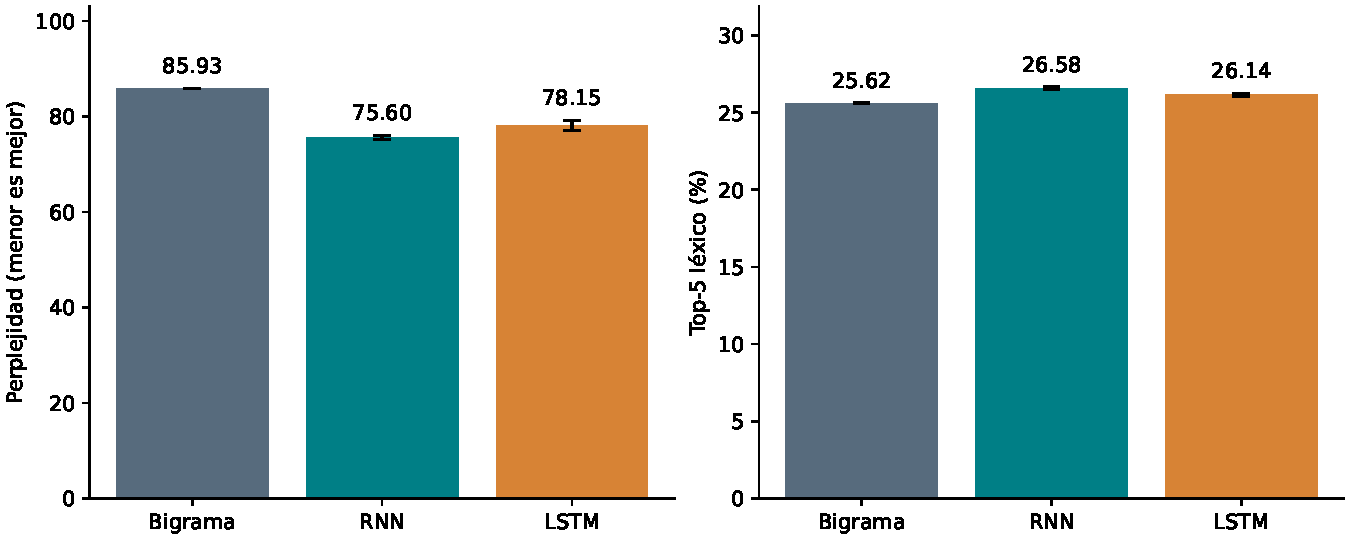
\includegraphics[width=.95\textwidth]{figuras/comparacion.pdf}
\caption{Perplejidad y top-5 de prueba. Las barras finas de las redes muestran desviación entre tres semillas, no incertidumbre sobre cualquier corpus.}
\label{fig:comparacion_nueva}
\Description{Dos gráficos de barras comparan bigrama, RNN y LSTM. La RNN tiene menor perplejidad y mayor top-5 en el protocolo ejecutado.}
\end{figure*}
La Figura~\ref{fig:comparacion_nueva} contiene dos gráficos. En ambos, el eje horizontal identifica los modelos. En el gráfico de la izquierda, el eje vertical corresponde a perplejidad; una barra más baja representa un resultado mejor. En el de la derecha, el eje vertical representa porcentaje top-5; una barra más alta representa mayor acierto.

Las pequeñas marcas negras encima de las barras de las redes muestran la variación entre semillas. Su poca altura en top-5 indica que los porcentajes de esas tres ejecuciones estuvieron próximos. No expresa ausencia de errores en las palabras: un modelo puede mantener resultados parecidos entre semillas y seguir acertando una proporción limitada de objetivos.

La figura facilita comparar visualmente los valores, mientras que las tablas permiten consultar números concretos. Ambas provienen de los mismos registros. No son dos experimentos independientes. Los colores distinguen modelos y no representan clases gramaticales, lenguas ni conjuntos de datos.

\subsection{Curvas de aprendizaje}
\begin{figure*}[tb]
\centering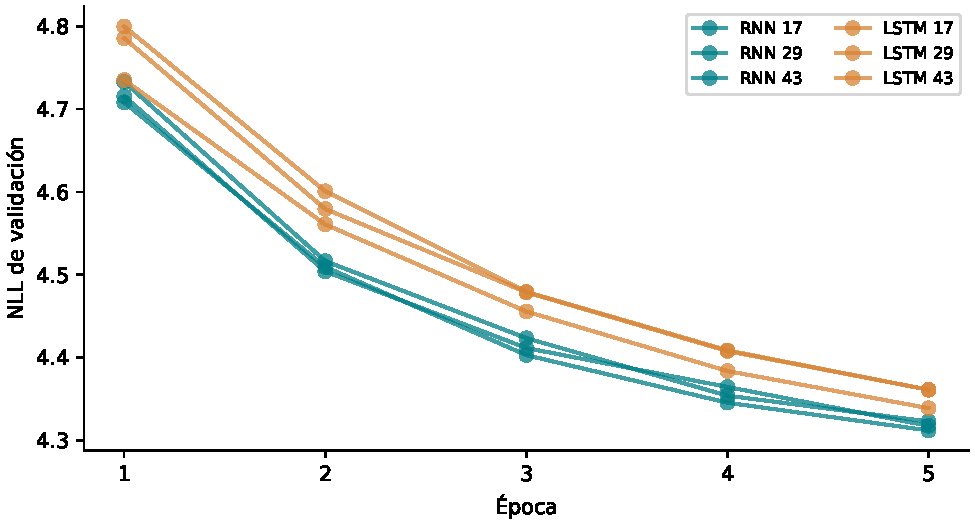
\includegraphics[width=.78\textwidth]{figuras/aprendizaje.pdf}
\caption{Pérdida de validación durante las cinco épocas del estudio principal. Cada línea corresponde a una arquitectura y una semilla.}
\label{fig:aprendizaje_nueva}
\Description{Seis curvas muestran una disminución de pérdida de validación durante las cinco épocas para RNN y LSTM.}
\end{figure*}
La Figura~\ref{fig:aprendizaje_nueva} usa el eje horizontal para indicar la época y el vertical para indicar NLL de validación. Cada punto resume todos los objetivos de validación de una época. Una línea une los cinco puntos de una misma ejecución. Las etiquetas 17, 29 y 43 son semillas, no números de palabras ni cantidades de capas.

Las curvas descienden a lo largo del entrenamiento observado. Esto indica que las versiones sucesivas asignaron mejor probabilidad a los objetivos de validación en ese tramo. No demuestra que el modelo haya alcanzado su mejor resultado posible. Para examinar qué ocurre con más épocas sería necesario un experimento adicional que no ajuste decisiones a partir de la prueba ya utilizada.

La figura representa validación, no prueba. Esta distinción es importante porque validación interviene en la selección del modelo guardado. Utilizar una curva de prueba para elegir la época mezclaría la selección con la evaluación final. El programa mantiene separadas esas dos funciones.

\subsection{Seguimiento de una ejecución completa}
Para concretar la lectura de las curvas, se presenta la ejecución LSTM con contexto doce y semilla 29, correspondiente al modelo seleccionado para la demo. La tabla siguiente muestra sus cinco épocas. Los datos proceden del historial guardado durante entrenamiento y se redondean únicamente para su presentación.

\begin{table*}[tb]
\caption{Historial observado de LSTM, contexto doce, semilla 29.}
\centering
\begin{tabular}{rrrrr}
\toprule Época & NLL entrenamiento & NLL validación & PPL validación & Top-5 validación (\%)\\\midrule
1 & 5.291 & 4.735 & 113.89 & 22.96\\
2 & 4.734 & 4.561 & 95.66 & 24.68\\
3 & 4.557 & 4.456 & 86.10 & 25.30\\
4 & 4.431 & 4.384 & 80.13 & 26.19\\
5 & 4.338 & 4.339 & 76.61 & 26.49\\\bottomrule
\end{tabular}
\end{table*}

La pérdida de validación disminuye de 4.735 a 4.339 en las épocas registradas. La perplejidad también disminuye y el top-5 aumenta. En esta ejecución, la quinta época tiene la menor NLL de validación, por lo que es la versión conservada. La tabla permite justificar esa selección sin recurrir al resultado final de prueba.

La pérdida de entrenamiento se acumula mientras el modelo está aprendiendo. Dentro de una época, los parámetros cambian después de cada lote. En cambio, la pérdida de validación se obtiene al terminar la época, con la versión de parámetros de ese momento. Por esta razón, no se deben interpretar sus valores como si fueran dos evaluaciones simultáneas de un modelo idéntico sobre datos intercambiables.

También cambia el modo de operación: dropout está activo mientras se entrena y se desactiva al evaluar. Las particiones poseen sus propias palabras y frecuencias. Una diferencia entre columnas, por sí sola, no demuestra que exista un error ni permite cuantificar toda la capacidad de generalización. Para interpretar sobreajuste se necesita examinar la evolución y el diseño, no exigir igualdad exacta entre pérdidas.

La primera época ya contiene muchas actualizaciones. Su resultado no representa una red completamente sin entrenamiento. Del mismo modo, la quinta fila no corresponde a una nueva arquitectura: conserva las mismas dimensiones y cambia los parámetros que aprendieron durante las pasadas anteriores. Los puntos de una curva describen versiones sucesivas de una ejecución, mientras que las semillas describen ejecuciones distintas.

El top-5 de validación de la última fila es aproximadamente 26.49\%. El top-5 de prueba de ese mismo modelo es aproximadamente 26.20\%. La diferencia responde a conjuntos distintos. No se reemplaza la cifra de prueba por la de validación para presentar un porcentaje mayor. Tampoco se promedian ambas particiones, porque sus funciones dentro del protocolo son diferentes.

La perplejidad de validación de esa fila es 76.61, frente a 76.94 en prueba para la ejecución seleccionada. Estos dos valores tampoco deben confundirse con la media de 78.15 de las tres LSTM principales. Existen tres niveles de lectura: una versión por época en validación, una ejecución seleccionada evaluada en prueba y un promedio de varias ejecuciones. Informar a cuál corresponde cada número evita aparentes contradicciones.

El seguimiento numérico complementa la figura y permite repetir una comprobación sencilla: localizar la menor pérdida de validación en el historial, consultar la época guardada del modelo y confirmar su identidad. No exige volver a entrenar para comprobar lo que ya quedó registrado. Una nueva ejecución independiente sería una comprobación adicional de reproducibilidad, distinta de verificar la coherencia interna de estos archivos.

\subsection{Efecto de la longitud de contexto}
\begin{table*}[tb]
\caption{Comparación exploratoria de contextos con semilla 17.}
\centering
\begin{tabular}{lrrrr}
\toprule Modelo & Contexto máximo & Perplejidad & Top-1 (\%) & Top-5 (\%)\\\midrule
RNN & 4 & 75.49 & 7.64 & 26.50\\
RNN & 12 & 75.21 & 7.88 & 26.57\\
RNN & 24 & 75.73 & 7.74 & 26.54\\
LSTM & 4 & 78.30 & 6.69 & 26.05\\
LSTM & 12 & 78.82 & 6.87 & 26.04\\
LSTM & 24 & 78.46 & 7.05 & 25.99\\\bottomrule
\end{tabular}
\end{table*}

En RNN, el contexto doce obtiene menor perplejidad que cuatro y veinticuatro para la semilla mostrada. En LSTM, el contexto cuatro obtiene menor perplejidad que doce y veinticuatro en esta comparación. No se observa que aumentar el contexto produzca una mejora continua de todas las métricas.

El resultado debe interpretarse con cautela porque cada contexto adicional tiene una sola semilla. No permite distinguir con suficiente detalle el efecto de la longitud de otras variaciones de entrenamiento. Tampoco prueba que una LSTM no pueda aprovechar dependencias largas: la tarea utiliza ventanas relativamente cortas, un presupuesto breve y texto natural cuya información relevante no se controló por distancia.

La fila con contexto doce de esta tabla corresponde únicamente a la semilla 17. No debe sustituirse por la media de tres semillas de la tabla principal sin avisar, porque se mezclarían niveles de resumen. Esta diferencia explica que aparezcan 75.21 y 78.82 aquí, mientras que la comparación principal presenta 75.60 y 78.15.

\subsection{Cobertura del vocabulario}
De los 56796 objetivos de prueba, 12033 se representan como UNK. Esto equivale aproximadamente a 21.19\%. Las posiciones restantes, 44763, corresponden a entradas identificables. Incluso si el modelo acertara todas esas posiciones conocidas, no podría superar aproximadamente 78.81\% de acierto léxico con la regla actual y sin ampliar su capacidad de producir palabras.

Ese límite no describe el acierto alcanzado, sino un máximo impuesto por la representación. El top-5 real es mucho menor. La cobertura explica una parte de la dificultad, pero no todas las predicciones incorrectas: también existen palabras conocidas que el modelo ordena fuera de los primeros lugares.

La perplejidad trata de otra manera estas posiciones porque utiliza UNK como objetivo interno. El modelo puede asignar probabilidad a esa categoría y recibir una pérdida limitada aunque no distinga el término original. Por eso la perplejidad de un vocabulario reducido no debe compararse sin más con la de otro sistema que represente todas las palabras de forma distinta.

\subsection{Cantidad de parámetros}
La RNN tiene 346296 parámetros y la LSTM 368184. La diferencia es 21888, aproximadamente 6.32\% respecto a la RNN. En ambas arquitecturas, la representación de palabras aporta 144000 parámetros y la proyección de salida aporta 195000. La parte recurrente contiene 7296 en RNN y 29184 en LSTM.

La diferencia total es menor de lo que podría esperarse al observar cuatro transformaciones recurrentes en LSTM, porque embedding y salida ocupan una parte grande del total y son iguales en ambas redes. Esto ayuda a interpretar el tamaño del modelo. Una mayor cantidad de parámetros no es sinónimo de mayor acierto y no describe por sí sola cuántas operaciones se realizan en cada consulta.

\begin{table*}[tb]
\caption{Distribución de parámetros de la configuración usada.}
\centering
\begin{tabular}{lrr}
\toprule Componente & RNN & LSTM\\\midrule
Embedding & 144000 & 144000\\
Parte recurrente & 7296 & 29184\\
Proyección final & 195000 & 195000\\\midrule
Total & 346296 & 368184\\\bottomrule
\end{tabular}
\end{table*}

\subsection{Tiempos de ejecución}
El tiempo medio de entrenamiento de las tres ejecuciones principales fue 78.17 segundos para RNN y 107.44 segundos para LSTM. Las cinco épocas y las evaluaciones de validación forman parte de ese tiempo registrado. La comparación utiliza CPU y dos hilos. No se interpreta como una garantía de duración en cualquier computadora.

Se midió también la duración del cálculo de una predicción con lote de un ejemplo, después de diez calentamientos y sobre cien consultas. La mediana indica el valor central de los tiempos ordenados y el percentil 95 indica el valor por debajo del cual se encuentra aproximadamente el 95\% de las mediciones. Estas mediciones excluyen carga del archivo, tokenización y escritura de salida.

La demo vuelve a cargar el modelo en cada consulta, de modo que la espera que observa la persona incluye actividades adicionales. Por eso el tiempo del cálculo interno no se presenta como tiempo total de respuesta de la aplicación. Para una evaluación de uso real se tendría que medir el recorrido completo y controlar la carga del equipo.

\subsection{Ejemplos observados en la demostración}
Con entrada vacía, el programa procesa la señal de inicio. La primera sugerencia registrada es ``el'' con aproximadamente 14.21\%. Le siguen ``la'', ``en'', ``los'' y ``pero''. La probabilidad de UNK es aproximadamente 10.95\%. Este caso permite comprobar que una entrada sin palabras se trata de forma definida y no produce una operación sin elementos.

Para ``el presidente del gobierno'', las sugerencias registradas son ``de'', ``del'', ``vasco'', ``es'' y ``se''. La palabra ``de'' recibe aproximadamente 13.77\%; UNK recibe 10.61\%. La entrada no contiene palabras desconocidas. Aun así, el programa no conoce la continuación que pretende escribir una persona y presenta varias opciones en lugar de una afirmación de corrección única.

\begin{table*}[tb]
\caption{Salida observada para ``el presidente del gobierno''. Las probabilidades conservan su valor dentro de la distribución completa.}
\centering
\begin{tabular}{lrr}
\toprule Candidata & Posición visible & Probabilidad aproximada\\\midrule
de & 1 & 13.77\%\\
del & 2 & 7.35\%\\
vasco & 3 & 3.00\%\\
es & 4 & 1.97\%\\
se & 5 & 1.97\%\\\bottomrule
\end{tabular}
\end{table*}

Para ``la universidad de'', la primera sugerencia es ``la'', con aproximadamente 10.74\%, y UNK recibe 20.02\%. La lista incluye la categoría numérica. El ejemplo muestra que una entrada completamente conocida no asegura que la salida resulte suficientemente específica para el uso esperado. La red puede favorecer términos generales y no producir el nombre concreto que una persona espera.

En ``los estudiantes de software'', la palabra ``software'' aparece como desconocida. La primera sugerencia es ``de'', con aproximadamente 7.53\%, y UNK recibe 22.05\%. Este resultado se relaciona con la lista de vocabulario utilizada, no con la afirmación de que el término no exista en español técnico. El programa solo informa que no dispone de una entrada propia para esa forma.

En ``Riobamba ESPOCH Chimborazo'', las tres formas normalizadas son desconocidas. La primera sugerencia es ``de'', con aproximadamente 5.07\%, y UNK recibe 24.64\%. El caso ayuda a mostrar la diferencia entre disponer de un modelo en español y reconocer vocabulario local concreto. No se puede atribuir a estas salidas un conocimiento comprobado de la ciudad o la institución.

Los ejemplos de demo se seleccionaron para explicar comportamientos. No constituyen una muestra aleatoria de todas las consultas posibles. Tampoco tienen una única palabra de referencia que permita contarlos automáticamente como acierto o error. La evaluación cuantitativa utiliza el conjunto de prueba; los ejemplos permiten examinar cómo se presenta el resultado a una persona.

\subsection{Qué permite concluir la comparación}
Las redes obtuvieron mejor perplejidad que el bigrama bajo el protocolo usado. La RNN obtuvo el mejor promedio principal de las métricas informadas. La mejora top-5 respecto al bigrama fue menor de un punto porcentual. Estas son conclusiones apoyadas por los valores registrados.

Una posible explicación de que LSTM no obtenga ventaja es que el tamaño de la muestra, las ventanas y las cinco épocas no favorezcan un aprovechamiento suficiente de su mecanismo de memoria. Sin embargo, el estudio no modifica cada factor de manera independiente para comprobar esa explicación. Debe presentarse como posibilidad, no como causa demostrada.

Las referencias sobre LSTM describen capacidades y resultados en otros escenarios. No obligan a que toda implementación local supere a una RNN simple. Conservar un resultado distinto de la expectativa permite mostrar una práctica de investigación adecuada: describir el experimento, informar los datos y limitar la conclusión a lo que se midió.

\subsection{Limitaciones del estudio}
La primera limitación es el vocabulario reducido y su alta proporción de desconocidas. La segunda es el dominio periodístico, que no representa todos los usos del español. La tercera es el presupuesto de entrenamiento: cinco épocas permiten una comparación concreta, pero no garantizan que cada arquitectura haya alcanzado su mejor configuración.

También existen límites de comparación. Usar la misma tasa de aprendizaje no significa que sea igualmente adecuada para ambas redes. Utilizar el mismo tamaño oculto no iguala cantidad de parámetros. Repetir tres semillas no sustituye repetir el experimento con varios corpus o divisiones. Estos puntos no invalidan las mediciones; delimitan la pregunta que realmente respondieron.

La separación por documento y la eliminación de duplicados exactos reducen riesgos de coincidencia entre datos, pero no eliminan noticias similares. La evaluación automática tampoco mide si una persona acepta una sugerencia. Un despliegue real necesitaría valorar errores de escritura, tiempos completos de respuesta, pertinencia de candidatos y comportamiento con vocabulario del entorno de uso.

\subsection{Relación con el propósito educativo}
La práctica permite seguir una cadena verificable: texto original, preparación, ejemplos, arquitectura, entrenamiento, evaluación y sugerencias. Esa relación es más importante para comprender el tema que memorizar una cifra aislada. Un integrante debe poder explicar cómo se obtiene el resultado y qué decisión cambiaría si se modifica una condición del experimento.

Las preguntas técnicas de la defensa pueden responderse a partir de esa cadena. La memoria se explica en el estado y la celda; las compuertas, en la actualización LSTM; la calidad predictiva, en las métricas; y la reproducibilidad, en las configuraciones y datos guardados. No es necesario introducir arquitecturas ajenas al tema para justificar el alcance del programa presentado.

\section{Conclusiones}
La predicción de la siguiente palabra permite estudiar de forma concreta el procesamiento de secuencias. El contexto aporta las palabras anteriores y el modelo asigna probabilidades a posibles continuaciones. La salida depende tanto de la arquitectura como de la representación del texto, el vocabulario y los ejemplos utilizados durante entrenamiento.

La RNN simple mantiene un estado oculto que se actualiza en cada posición. La LSTM añade una celda y compuertas que regulan la retención, la incorporación y la salida de información. Esta diferencia explica su mecanismo de memoria, pero no garantiza una mejora automática en cualquier experimento. En la implementación, ambas arquitecturas reinician sus estados por ventana y solo acceden a los elementos incluidos en ella.

Se construyó un procedimiento que utiliza documentos separados para entrenamiento, validación y prueba, un vocabulario común de 3000 entradas y 100000 objetivos seleccionados para aprender. El programa implementa las dos redes, una referencia de bigramas, métricas y una demo. Las pruebas de integridad verifican propiedades de preparación, evaluación y recuperación del modelo necesarias para interpretar la ejecución.

Sobre 56796 objetivos de prueba, la RNN obtuvo perplejidad media de 75.60 y la LSTM de 78.15, frente a 85.93 del bigrama. El top-5 léxico fue 26.58\%, 26.14\% y 25.62\%, respectivamente. La comparación favorece a la RNN en las condiciones fijadas y muestra una mejora limitada del acierto en las primeras cinco posiciones. No demuestra superioridad general de RNN sobre LSTM.

La tasa de desconocidas de 21.19\% restringe la capacidad de identificar palabras concretas. Los ejemplos de la demo muestran esa limitación con términos del entorno local y del área de software. El sistema es útil para estudiar recurrencia y evaluación, pero los resultados no respaldan presentarlo como un autocompletador de amplia cobertura listo para un uso productivo.

La perplejidad y el acierto deben interpretarse conjuntamente. La primera resume probabilidad asignada a los objetivos, incluida la categoría desconocida; el segundo exige identificar una palabra conocida en una posición determinada. Diferenciar ambas medidas evita confundir una mejora de probabilidad con un aumento equivalente de palabras acertadas.

Como extensión del mismo problema, se podría estudiar un vocabulario de mayor cobertura, un presupuesto de entrenamiento diferente o más repeticiones de la comparación de contextos. Esas propuestas requieren nuevos protocolos y evaluaciones independientes. No forman parte de los resultados realizados ni se utilizan para sustituir las limitaciones del experimento actual.

\section{Enlaces a recursos}
El código del proyecto está organizado en scripts de Python y los registros permiten consultar las métricas sin redondear. La guía de aprendizaje complementaria explica las rutas, los comandos y la procedencia de cada elemento. Las direcciones públicas del repositorio y de la presentación se incorporarán cuando los recursos estén publicados y se haya comprobado su acceso. No se presenta una dirección no creada como si estuviera disponible.

El corpus utilizado puede consultarse en
\url{https://github.com/UniversalDependencies/UD_Spanish-AnCora/tree/r2.17}.
Los enlaces gratuitos a las doce publicaciones se encuentran en las referencias y en la guía complementaria. La presentación queda fuera de la revisión actual por indicación del grupo.


\bibliographystyle{ACM-Reference-Format}
\bibliography{referencias}
\end{document}
